\documentclass{ieeeaccess}
%\IEEEoverridecommandlockouts
% The preceding line is only needed to identify funding in the first footnote. If that is unneeded, please comment it out.
\usepackage{cite}
\usepackage{amsmath,amssymb,amsfonts}
\usepackage{algorithmic}
\usepackage{graphicx}
\usepackage{textcomp}
\usepackage{xcolor}
\usepackage{graphicx}

\usepackage{amssymb}
\usepackage{amsmath}
\usepackage{xcolor}%定义了一些颜色
\usepackage{colortbl,booktabs}%第二个包定义了几个*rule
\usepackage{multirow}
\usepackage{booktabs}
\usepackage{threeparttable}
\usepackage{amsmath}
\usepackage{caption}
\usepackage{subfigure}



\begin{document}
	
\history{}%Date of publication xxxx 00, 0000, date of current version xxxx 00, 0000.
\doi{}%10.1109/ACCESS.2017.DOI

\title{A Nearest Neighbor Similarity Method for Adversarial Samples Detection}


\author{\uppercase{Yi Ren}\authorrefmark{},
\uppercase{Xia Xie\authorrefmark{}, 
Hai Jin}\authorrefmark{},
\IEEEmembership{Fellow, IEEE}, and
\uppercase{Hanhua Chen}\authorrefmark{}
}
\address[]{National Engineering Research Center for Big Data Technology and System
	Services Computing Technology and System Lab
	Cluster and Grid Computing Lab
	School of Computer Science and Technology
	Huazhong University of Science and Technology, Wuhan, 430074, China}

%\tfootnote{This paragraph of the first footnote will contain support information, including sponsor and financial support acknowledgment. For example, ``This work was supported in part by the U.S. Department of Commerce under Grant BS123456.''}

\markboth
{Author \headeretal: Preparation of Papers for IEEE TRANSACTIONS and JOURNALS}
{Author \headeretal: Preparation of Papers for IEEE TRANSACTIONS and JOURNALS}

\corresp{Corresponding author: Xia Xie (shelicy@hust.edu.cn)}

\begin{abstract}
	%近邻算法是一个简单的无参数无训练过程的有监督分类算法,最早起源于1950年代。因为近邻分类算法没有像其他的机器学习算法那样有一个复杂的漫长的迭代训练过程过程,简单透明,性能高效,在二分类问题中有很好的性能,如今已经运用在了很多的领域当中,例如数据挖掘,模式识别,推荐系统等等。
	%由于近邻算法没有训练过程,测试数据样本的分类过程主要是需要和数据集中的收集好的样本进行相似度的计算,以此来作为分类的依据。近邻算法因此对于训练数据集,包括数据集的大小以及数据样本的特征维度和邻居节点相似度的计算要求较高。
	%目前,有很多的工作集中在如何快速的进行邻居节点的计算,例如并行分布式的计算框架,基于空间分解 recursive hyperplane decomposition 的加速方案,以及精简数据集,降维的方案。
	%但随着深度学习的快速发展,尤其是以生成模型为主的GAN模型的发展,人们现在可以利用数据的分布规律人为的制造出来各种各样的合成图片,对抗样本等,给当下的传统机器学习算法带来了很大的冲击,对抗样本对于分类的性能影响很大,而目前有关近邻算法的鲁棒性研究以及如何防御及检测这些对抗样本的工作还是有限的,因为近邻算法的运用场景很广泛,因此很有必要去分析和解决以上对抗样本带来的影响。
	%本文针对以上的问题,我们分析了训练数据集的鲁棒性表示以及近邻相似度的鲁棒性计算,提出了一种新的基于深度特征的以及特征子空间相似度计算的检测对抗样本的二分类方法。深度特征是将样本通过深度网络转换抽取,提取出中间层的新的特征表示,然后利用不同于精简数据集的方法对特征进行降维操作,最后通过基于特征子空间的distance and direction metric去发现待测样本的近邻节点,来检测出对抗样本。
	The $k$ nearest neighbor algorithm is a non-parametric supervised classification algorithm with no training process. Because the process of the classification algorithm does not have a complicated iterative training process compared with other machine learning algorithms, it is simple and transparent, and its performance is quite well in practice. 	
	However, with the rapid development of deep learning, especially the development of generative model such as GAN, people can now use the distribution of data to artificially create a variety of synthetic datas, adversarial samples which results the final misclassification. It has brought a huge impact to the current traditional machine learning algorithms. Adversarial samples have a great impact on the performance of classification. At present, the research on the robustness of $k$ nearest neighbor algorithm is limited. 
	In this paper, we analyze the representation of data samples in the different feature space, including the data sample dimension reduction method such as GEM and LFDA, and the deep learning method to transform the original feature space to low dimension and abstract represention. Experiments show that the representation of data samples in different feature spaces will have different robust performance to adversarial samples, the improved subspace nearest neighbor similiarity algorithm are used to detect the potential adversarial sample among correctly classified true samples. These can effectively detect the misclassified threatened instance and ensure the reliability of the classifiers.
\end{abstract}

\begin{keywords}
nearest neighbor search,  adversarial samples,  data mining
\end{keywords}

\titlepgskip=-15pt

\maketitle
\pagestyle{empty}  % no page number for the second and the later pages
\thispagestyle{empty} % no page number for the first page

\section{Introduction}
%KNN分类算法的问题:1.两类数据存在明显的边界情况下,在内部分类效果很好;但是在分类边界处的分类效果急剧下降;
%KNN分类算法的问题:2.所以会有其他的分类算法出现,例如逻辑回归,寻找分类的边界曲线而不是直线;逻辑上回归的算法,即预测数值,但实际上是用来分类的任务。

%平方损失函数的问题:主要两个问题,一个是算法模型中存在指数型,平方后可能非凸,另一个是直接相减的方式不能体现足够明显的惩罚和奖励;
%平方损失函数的问题:1.线性回归问题中,参数只有w和b,使用平方损失函数后,参数的次数变成2次,是为了构造出来凸函数,从而可以使用偏导数为零进行求解参数;但是在其他的模型下,如逻辑回归的模型下,参数本身可能不是一次线性的,使用平方损失函数后也不会构造出凸函数,从而不是借用偏导数的方法求解参数。
%平方损失函数的问题:2.在以阈值作为分类准则的情况下,例如0.5,计算结果0.51的情况下,正确的误差有(1-0.51)^2,错误的误差有(0-0.51)^2,计算出的损失都很大(分类正确的情况下,奖励不明显),(损失函数模型)需要的是在分类正确的情况下,损失快速减小(明显的奖励);分类错误的情况下,损失快速上升(明显的惩罚)。

%对数损失函数作用:1.用来抵消指数,变成系数的一次项表达式;2.自变量在(0,1)区间上时,对数函数的变化最敏感,lg(x),当x小于0.5时,lg(x)急速减小;
%对数损失函数需要经验风险的结构化,引入正则化项:系数的一次项表达式求最小值不保险,引入一个系数的二次项作为正则化项,构造出凸函数,再求最小值。
\label{sec:introduction}
\PARstart{W}{e} are living in a world that a variety of data are produceed every day. It is ubiquitous that people have to process these big data to obtain the patern they want.
The $k$ Nearest Neighbor algorithm (KNN) is one of the data mining algorithms widely used in many fields that can automatically classify unlabeled sample $x$. It searchs the most similar $k$ neighbors of the unlabeled input sample $x$ in the training data set feature space and assigns the label which the most present among  neighbors to this sample $x$\cite{cover1967nearest}. 
At present, there has been a lot of work to optimize the efficiency and accuracy and their varients, e.g., weigh different neighbors specific weights\cite{bicego2016weighted} and dynamic $k$ nearest neighbors in replace of fixed $k$\cite{Zhong:2017:IKC:3055635.3056604}.
However, KNN is a data-driven model with no prior hypothetical modeling process and distinguishes sample internal relationships based on the spatial feature distance between samples, the distribution and multi-modality of data samples will have a large impact on classification decision. Therefore, adversarial exsamples will bring huge threats to the KNN model.

%对抗样本的特点是在通过向原始的数据特征中添加干扰,使得分类模型最终分类错误。添加的扰动一般都是精心计算过的,对于我们肉眼来说基本难以察觉,但是对于分类器确实灾难。
Adversarial samples are characterized by finding as few disturbances as possible, and these disturbances are imperceptible to the observer but it is really a disaster for the classifier \cite{goodfellow2014explaining}. Adversarial samples have been shown to be transitive across different similar network architectures, as well as transitive between networks trained on different subsets of data. The KNN model is an important basic component of other discriminant model and used in many areas with high requirements for safety performance, for example, in the field of autonomous vehicles, someone can intentionally alter a normal danger warning sign slightly, this attack is so negligible to detect by human eye, and misclassified to another innoxious sign by the classification model. It is very common in the field of patern recognition but leading to serious consequence.

Currently, there is a little amount of work focused on the adversarial sample to KNN models. The method proposed in\cite{wang2017analyzing} mainly analyzes distributional properties and data samples size on robustness, proposing a method of changing the state of the original data set to resist the attack of the adversarial examples. This work theoretically deduce the impact of the data size and the values of $k$ on the robustness of the classifier model, which requires complex calculations of the original data set in advance.
Another research direction of KNN classifier is to reduce the dimensionality of the data and compress the data into a smaller feature space\cite{lin2011parameter}, so that the data can be more dense and better to represent the original distribution of the data. However, the adversarial samples can be distingished in the original dimensional space, which will be compressed into "normal" samples in the low dimensional because singularity disappears and brings more serious problem. 
So just reducing the dimension is not enough, we need more rigorous and abstract data representation. 

Deep learning is essentially a feature extraction process \cite{gordo2016deep}. It passes the original input data through a multi-layered learning structure model to obtain a layer-by-layer transformation of the data features , numerous neurons can transform the original data samples into a more abstract and flexible feature space and finally obtains the deep feature expression of the data, and could dig out novel feature representations that are difficult to mine by traditional matrix decomposition methods.
Based on the deep feature space, we perform nearest neighbor similarity search in the subspaces of each class, taking training samples into consideration as much as possible.  Finally, based on the trade-off consideration and analysis of similarity score of each class to determine the input sample, we can judge whether is a adversarial sample. 

%目前的主要分类方法是将数据进行降维操作[Nearest Subspace with Discriminative Regularization for Time Series Classification],将数据压缩到一个更小的特征子空间中去[k-NS: A Classifier by the Distance to the Nearest Subspace],这样使得数据能够更加的密集,更好的去表现数据的原始分布,但是这样的操作能够带来计算上的便利和效率,也会牺牲部分的准确性,更加严重的是,经过压缩,本来在高维空间中的对抗样本也会被压缩成了“正常”的样本,带来更加严重的问题。

	The main contributions of this paper are as follows: 
\begin{itemize}
	\item 
	Firstly, continue to study and expound the influence of adversarial exsamples on the parameter-free machine learning algorithm such as KNN algorithm, and propose a new KNN method model to use the hidden layers activations of deep feature for neural network to detect and process the adversarial exsamples.
	\item 
	Secondly, the distance between two instance samples in the feature space can reflect the similarity degree. The feature space of the KNN model is generally the n-dimensional real vector space $R^n$. Euclidean distance is commonly used to calculate the distance between data samples in feature space, a more general calculation formula is $L_{p}$ distance. Besides, tangent distance is a distance measure that is not sensitive to transformations (such as translation, rotation, scale transformation, etc.) and is used to replace the traditional euclidean distance. \cite{simard1998transformation}. Based on the above considerations, a measurement method different from directly calculating the distance between neighbors is adopted. Calculating the feature space of the samples to be classified for each class is used as the similarity calculation method. We realize that the original KNN does not take into account the limitations and complexity of the training data set feature space, so in this paper we performs neighbor search and analysis the subspace of each class and finally consider all the similarity scores of each classes to achieve a robust KNN moedl. 
\end{itemize}

%一是通过GAN模拟现有的数据分布,得到更多的数据来丰富训练数据集,使得在待测instance周围有足够多的/密集的正常样本存在;
%二是由于不同的距离度量的方法得到的邻居会存在差异,例如LP距离当p取不同的数值时,覆盖的领域面积是不一样的,基于以上的考虑,采用不同于直接计算邻居间距离的度量方式,采用计算待测instance到每一个的类别的特征空间的方式来作为相似度的计算方式,这样一方面可以减少计算的复杂度,另一方面还可以对对抗样本有一定的防御,比较的是样本和特征空间超平面()具体的特征空间形式取决于k值)之间的距离,而不是直接的样本之间的距离,使得对抗样本的攻击减弱;
%三是通过核函数将已有的数据的特征向量向高维空间映射,使得本来在低维空间接近的对抗样本能加的稀疏和分散,同时得到一些线性不可分的隐变量,提高算法的分类准确性和鲁棒性。

This paper is organized as follows. Section2 reviews the state-of-the-art related work. Section3 gives an overview of the technical challenges and then presents the our method's architecture. Section4 presents the methodology in detail. We give an evaluation of in Sect.5. Finally, we draw an conclusion and indicate some directions for future work.



\section{Related Work}
%KNN分类算法的问题:1.两类数据存在明显的边界情况下,在内部分类效果很好;但是在分类边界处的分类效果急剧下降;
\subsection{Works on Nearest Neighbors}
The setting of the KNN algorithm is very simple and efficient, and does not require training parameters. It was first proposed by T. M. Cover and P. E. Hart for the classification problem\cite{cover1967nearest}. KNN algorithm is listed as one of the top ten machine learning algorithms and one of the necessary algorithms for learning machine learning.

There are a lot of optimizations about KNN \cite{cover1967nearest}, most of these tasks focus on improving the efficiency of the KNN algorithm and the accuracy of the classification \cite{chaudhuri2014rates}. KNN is a regression method that does not require training parameters. Usually, the value of $k$ can be set according to the size of the data set empirically and $k$ is fixed. \cite{Zhong:2017:IKC:3055635.3056604} proposes an improved KNN algorithm, which is indicated as Dk-NN, by using an interval of parameter $k$ in replace of fixed parameter $k$, and obtain variation tendency curves under different $k$ values to assist decision-making.
The article \cite{bicego2016weighted} proposes a weighted KNN method: when performing neighbor space metrics,it sets different weights for different neighbors, and design a pool of classifiers with different weights. The classifier group finally determines the final classification result based on the weighted result of the boost classifiers to improve the classification accuracy.

In addition to considering the selection of the $k$ value and the weighted metric scheme for the KNN algorithm, there are some methods that focus on establishment a spatial index structure to speed up the process of comparison and calculation \cite{zhang2017efficient}. 
In a pattern classification problem, it usually involves the use of high-dimensional feature data, which can easily make the classifier very complicated and time-consuming, another solution is to optimize the data sample feature space and data set. Irrelevant or redundant features will increase the complexity of the classification process and consume more resources and time to complete the classification task, and it is likely to reduce the classification accuracy of the classifier \cite{lin2011parameter}. In \cite{guyon2003introduction}, the importance of feature selection for discriminant models is analyzed, and some common methods are introduced. Some researchers are committed to streamlining and transforming the data set to improve the retrieval efficiency and convergence of traditional KNN classification \cite{draszawka2015improving} \cite{pawlovsky2014method}. \cite{shi2011improved} deal with the imbalance of data samples based on the distribution density of the data samples. Earlier research on the robustness of KNN used soft labels instead of crisp labels to classify and solve the problem of overlapping classes between data samples \cite{el2006study}.
%KNN算法的设定十分简单和高效,不需要训练参数,首次是由T. M. Cover and P. E. Hart for the  classification problem [4].提出来的。并且KNN算法在实际应用中十分的广泛,被列为十大机器学习算法之一,是学习机器学习的必学算法之一。	
%关于KNN有很多的优化工作,例如。。。但是这些工作大部分都是考虑到了KNN算法的执行效率和分类的准确。KNN算法是一个无参数的机器学习算法,In the k-NN algorithm, k is the only parameter and often set to a fixed value empirically.,例如在 Improved k-NN Classification with Dynamic k[]文章中,作者 proposes an improved k-NN algorithm, which is denoted as Dk-NN, by using dynamic k in replace of fixed k value.
%文章[Weighted K-Nearest Neighbor Revisited]提出了一种加权的KNN方法,在进行邻居的space metric的时候,为不同的nearest neighbor设定不同的weight,并且设计a pool of classifiers具有不同权重计算的KNN分类器组,最终根据这一组分类器的加权分类结果来确定最终的分类结果,来提高算法的分类accuracy。
%除了考虑到KNN算法的K值的选取和加权度量scheme,还有一些方法着重考虑对训练数据集建立高效的数索引结构[Efficient kNN Classification With Different Numbers of Nearest Neighbors],这样在查找近邻的时候就不用检索数据集中的全部训练数据,减少了查询的时间。
%还有的方案是Managing feature space or sample datasets; 对数据集中的数据进行降维和去冗余的操作。
\subsection{Works on Adversarial Samples}	
As the Iran Good fellow et al. first proposed and defined the adversarial sample, by adding a small amount of perturbation to the original data, then the modified data and the original data were used to derive different classification labels \cite{goodfellow2014explaining}. Such as it is jammy for the human to recognize a picture of a dog with minor changes without interference, this change is sensitive to the classifier, and the classifier incorrectly classifies it into a cat resultly. The main research work on current adversarial samples can be divided into two kinds:one is how to generate adversarial samples and the other is to defense against adversarial samples. Regarding the defense work against the adversarial sample, in the robust research work of the algorithm model, most of the current research on the adversarial sample is concentrated on the network \cite{wang2017analyzing}. 

At present, the latest research on parameter-free machine learning algorithms such as KNN is still rare \cite{zugner2018adversarial} \cite{wang2017analyzing}. However, the system analyzes different data sets robust and the algorithm's robust. It takes a huge computational cost to get the final robust NN algorithm, and real-time performance is difficult to guarantee. In this paper, different research methods are proposed. Through the deep feature and redesigned nearest subspace-based metrics, an efficient robust KNN algorithm is implemented to detect adversarial samples.

%随着Iran Good fellow等人首次提出和定义了对抗样本,通过对原始数据添加小部分的扰动,然后就会倒是改动后的数据和原始数据得出不同的分类标签[],比如说人的肉眼可识别的一张猫的图片,通过添加了对抗攻击的扰动后,分类器会将其分类成狗。当前的对抗样本的主要研究工作可以分为生成对抗样本和防御对抗样本。关于对抗样本的防御工作,算法模型的robust研究工作中,目前大部分关于对抗样本的研究都是集中在network上的。目前最新的关于无参数的机器学习算法例如KNN上的研究还很少,最新的工作就是文章[Analyzing the Robustness of Nearest Neighbors to Adversarial Examples]中就针对KNN由于其无参数的设定,因此算法的分类效率特别的依赖于训练数据集的robust性能,从训练数据集上进行robust设计,较为系统的分析了KNN算法中robust概念和设定,并根据作者的设定,提出r分子集的算法,提高了KNN算法在adversarial sample上的性能。但是系统的分析不同的数据集robust以及算法的robust,得到最终的robust NN算法需要花费巨大的计算代价,实时性也难以保证。本文的提出不同的研究方法,通过deep feature和重新设计的基于最近子空间的度量方法,来实现高效的robust KNN算法,检测adversarial sample。

\section{Background And Problem Statement}
\subsection{KNN Basic Theory}
The main process of classification of $k$ nearest neighbor is as follows:
%KNN算法的主要分类过程是这样的:首先需要一个training dataset $D_{train}$	
%D中的每一个x就是M维特征空间中的一个点,描述现实生活中的一个具体的instace,y就是x对应的标签,在二分类的任务中y=1or0.
given a dataset $D_{\text { train }}=\left\{(x, y) : x \in R^{N}, y \in Y\right\}$, the feature space of KNN model is generally N-dimensional real vector space $R^{N}$,
each $x$ in $D_{train}$ is a point in the N-dimensional feature space $R^{N}$, describing a specific instace in real life, $y$ is the label corresponding to $x$, and $Y$ = 1 or 0 in the task of the binary classification problem. 
for each sample $x_{i}$, $x_{j}$ in the dataset $D_{train}$, the $L_{p}$ distace between samples that represent the similiarity is difined as $x_{i}, x_{j} \in D_{train}, \quad x_{i}=\left(x_{i}^{(1)}, x_{i}^{(2)}, \cdots, x_{i}^{(n)}\right)^{\tau}, x_{j}=\left(x_{j}^{(1)}, x_{j}^{(2)}, \cdots, x_{j}^{(n)}\right)^{\tau}$:

\begin{equation}
L_{p}\left(x_{i}, x_{j}\right)=\left(\sum_{l=1}^{n}\left|x_{i}^{(l)}-x_{j}^{(l)}\right|^{p}\right)^{\frac{1}{p}}
\end{equation}
and find ordered $k$ nearest neighbors with the smallest $L_{p}$ distance:
\begin{equation}
Neighbors(x, X)=\left\{\left(x_{1}, y_{1}\right) \ldots\left(x_{k}, y_{k}\right)\right\}
\end{equation}

%当然,距离越远的数据之间,互相的影响就会越小,但是,多模态的数据却说明即使是症状不同的表现,最终也可能是同一种疾病。knn基于的假设就是说,同一个类的数据,一定都会是在一个局部的范围之内,不同类别的数据一定是在不同的范围之内。这种假设在一些数据集上可能有效,也被证实了,但是也存在一些特定的数据集,使得knn的这种假设变得低效,即一个类的数据在特征空间种存在不同的集群。

Of course, the farther away among the samples, the smaller the mutual influence is. But the multimodality data shows that even though samples from the same class may have a large distance in the feature space with each other. For example, a disease such as the cold, with multiple possible symptoms (e.g. fever, runny nose, joint pain), the special symptoms are different clusters within the same class. KNN is based on the assumption that the data of the same class must be within a local scope, and the data of different class must be within different range. This assumption may be valid on some datasets, and it has also been confirmed. But there are also some specific scenes that make this assumption of KNN inefficient, that is, one of the class of data exists in different clusters in the feature space. Therefore, we can not be neglected this characteristic of the data when doing the classification task. We try to take all samples in each class into considerration.	


%knn算法是一种简单的基础的机器学习算法,主要运用在分类、模式识别、目标检测等领域。knn算法的主要特点是:简单,算法中不需要其他的参数,唯一需要确定的是k值,通过确定k值来固定邻域的大小,k值的选取一般不能过大,否则knn这个算法模型会忽略更多的样本间的差异,使得模型变得简单,当k值设置为训练数据集大小的时候,对于每一次的分类任务,只会有一个固定的输出,即数据集中某一类样本数量最多的那个类的标签,
%虽然理论上证明当k最够大到 $\Omega(\sqrt{d n \log n})$时,对于对抗样本有很好的鲁棒性,但是这样的k值太大了而不能在实际中使用[5],同时k值也不能过小,否则一些噪声、异常值或者是对抗样本就会对分类造成很大的干扰,目前主要有动态k值等方法,本文主要采用的方法是交叉验证,通过多次实验比较,选择最适合的k值;其次规定好了领域的范围,就需要通过比较待测样本和数据集中的每一个样本来确定邻居,这是knn算法的关键,也是很多工作主要研究的部分,目前的主要研究工作是通过降维方法,将原始空间可能稀疏的数据压缩到更加密集的特征子空间中,通过在特征子空间中比较加工后的数据间的lp距离或者是待测样本到每个类所有样本张成的超平面的距离来确定最终的标签,但是通过我的调研和研究发现,这种方法并没有考虑到对抗样本存在的情况,但数据密集的时候,不仅会得到更加显著的特征表示,同时,向快速梯度下降等产生对抗样本的攻击也会更加容易干扰模型,因为本来就是在正常的样本上进行轻微的扰动来产生对抗样本,这样正常样本和对抗样本在空间距离上就是接近的,通过降维压缩,只会让恶意的对抗样本和正常样本更加接近,导致分类错误.


\subsection{Attack model for adversarial samples}
%给定一个定义好的数据集合,其中样本的特征向量和类别标签一一对应,攻击的目标就是通过对待测样本(没有对应标签)的轻微改动sample A -> sample A',来导致最终的分类预测性能下降,通过修改样本的特征来产生新的样本的方式叫做特征攻击,对于本文使用的数据来说,一般都用到的是特征攻击方式,对于其他的数据类型,例如图结构的数据,除了相应的特征攻击还有结构上的攻击,但是在本文中用不到。在待测样本的领域内修改部分邻居属性。
%我们的目标是对于具体的待测数据样本x,使得在原数据集上的分类预测结果和修改后的数据集上的预测结果不一样,当然由于数据间的关联关系,我们不能够仅仅是修改单一的数据样本点就能达到攻击的效果,因为x是在一个邻域内进行分类的,领域内的数据都会对最终的分类产生影响,因此,攻击者为了达到攻击的目的,不局限于只是对x产生扰动,同时也包括数据集中的其他样本。这样的情景也和现实生活中一致,一个想要去制造混乱的攻击者当然不会掌握所有的数据都有了解,也不是一个孤立单一的数据,往往是一部分的数据,根据这一部分数据来达到目的。受到[]启发,我们可以设置一个攻击的半径$r$,和攻击的预算,即在攻击半径内产生的扰动的多少$\Delta$,来限制产生的新数据集合和原始的数据集合足够的相似,不能和原始的数据产生太大的变异,不能完全的修改了原始数据,但是分类性能确有显著下降。
The generated adversarial sample model \cite{szegedy2013intriguing} can be defined as: given the normal input data sample $x$ , such as a digital image, and a trained classification discriminant model expressed as $y = f(x)$, after adding noise perturbations $\eta$ to the normal data sample $x^{\prime}$ ($x^{\prime} = x+\eta$) that are hard to detect by human eys, the target classification discriminant model misclassified $f(x+\eta) \neq f(x)$.

%对抗样本的生成可以根据是否针对特定类别而分为针对性攻击和非针对性攻击。 有针对性的攻击是生成对抗性样本并使分类判别模型将其分类为指定类别,而无目标的攻击是指使分类模型错误分类而又不关心分类结果的对抗性样本。
The generation of adversarial samples can be divided into targeted attacks and non-targeted attacks according to whether it targets a specific category. Targeted attacks are to generate adversarial samples and make the classification discriminant model classify them into a specified category, while non-targeted attacks refer to the adversarial samples that make the classification model misclassified without caring about the classification results.

A typical target attack adversarial method is under a bounded constraint L-BFGS algorithm \cite{byrd1995limited} to generate adversarial samples for targeted attacks. The author proposes a bound constrained optimization problem \cite{tabacof2016exploring} to obtain the smallest adversarial perturbation $\eta$:
\begin{equation}
\eta = {\underset{\eta}{\operatorname{minimize}}} ||\eta\|_{2}+L\left(x_i+\eta, i^{\prime}\right)\text { s.t. } x_i+\eta \in [0,1]^{m}
\label{L-BFGS}
\end{equation}
where $x_i$ represents the original data samples with label $i$, $\eta$ is the noise values of added perturbations to the normal data samples and $L( , )$ is the cost function computed between the original instance with class $i$ and the generated target class $i^{\prime}$ (different from the original image category $i$). Searching for an approximate solution to this problem, we can find the adversarial perturbations that makes the classifier classify as the target class and is hardly noticeable by human eyes.

Ian Godfell et al. \cite{goodfellow2014explaining} proposed the Fast Gradient Symbol Method (FGSM) to directly and quickly calculate the adversarial perturbation based on the linear characteristics in high-dimensional space. It is a typical non-targeted attack model that calculates all feature dimensions gradient of the input data to obtain the maximum adversarial disturbance.
The main idea of the algorithm: calculate the model gradient and then obtain the function related to the weight vector $w$. The loss will increase when each pixel variable value moves a small distance in the direction of its gradient, and then there will be a maximum change in the classification results. The sign function ensures that the direction of change is consistent with the direction of the gradient. 

Specifically, the problem can be modeled as follows Eq. \ref{FGSM}, where $\nabla_{x}$ is the gradient direction of parameter for the classification model, $y$ the desired target class related to the input data sample $x$, and $J(,)$ is the loss of the classification model. Although the change in each dimension is small, as the dimension increases, we can generate adversarial samples in the direction of increased loss, which will cause misclassification different form the desired target class. The cost function can be linearized near the current value of $ \ theta $ to obtain the optimal max-norm constraint perturbation \cite{carrara2017detecting}:
\begin{equation}
\eta = \varepsilon * \operatorname{sign}\left(\nabla_{x} J(x, y)\right)
\label{FGSM}
\end{equation}
It should be noted that the gradient can be calculated more easily by using the back propagation process of deep learning, so as to obtain the disturbance variable $\eta$ and $\epsilon$ is the hyperparameters controlling the magnitude and fooling power of the added perturbations. The adversarial input is a linear combination by $x^{\prime}=x+\eta$.

\subsection{Deep feature selection}
%数据的压缩技术、特征的降维的技术,从表现上来看都可以划分到数据的重新表示上来,将数据的在原坐标系下的原始表示或者是标记,通过迁移、映射等到一个维数更低的坐标系下表示,但是尽可能的保留数据之间的相互关系和内在联系,不破坏数据的信息。目前主流的方法有:PCA降维、word embeding、矩阵分解等。深度学习自从14年开始,研究的热度就在一直高涨,是由于深度学习能够将数据抽取到更加抽象的表示层面上,这些表示可能远远的脱离了人类的认识,所以会存在特征难以解释或者理解的问题,但是实验的结果都表表明,通过多层的神经网络抽取的特征,最终在分类上有很好的效果,这些抽象的特征适合计算机和算法的使用,目前也有一些研究工作利用深度学习学到的deep feature实现分类、模式识别等工作,取得一定的成果。
Feature selection is generally given an original feature set, from which a subset of features is selected to represent the original features, so that based on the improved representation the best classification results are achieved on classification models. Irrelevant or redundant features will increase the complexity of the classification process and consume more resources and time to complete the classification task, and it is likely to reduce the classification accuracy of the classifier. Therefore, for general pattern classification problems, feature selection is very necessary.
The compression and technique of dimension reduction of features can be considered as the representation of data sample, mapping data into a lower dimension without destroying the internal relevance information of the data samples. 
A typical application is processing time series data \cite{zhang2018nearest}. The features under the new representation have better distinguishing characteristics and improve the classification performance.
There are some other feature processing methods: PCA dimensionality reduction, word embeding\cite{gao2018self}, matrix decomposition \cite{karampatziakis2013discriminative} and so on. 

Deep learning is essentially a model of feature extraction as a subset of deep learning representation learning methods. It can automatically extract different levels of feature sets from the original data through the greedy algorithm's layer-by-layer training strategy, and these feature sets represent different levels of abstraction in the original data with special concept and meaning due to the development of back propagation technology.
Deep learning is a feature learning model that can automatically extract excellent features from the original data and has achieved great success in the fields of images, speech, text and so on. Through deep learning, you can get features at different depth levels from the original input data. And through such a deep learning process, the original input The data information hidden in the data can be extracted and abstracted layer by layer. The deeper the number of layers, the deeper the data concept represented by the extracted features is, which cannot be expressed and obtained by the shallow structure.

The trained neural network is used to extract the deep features containing the semantic information from the original data samples to obtain a reliable training sample feature set. These representations may be far removed from human understanding \cite{sani2017learning} but the results of the experiment show that the features extracted by the multi-layer neural network finally have a good effect on the classification \cite{chandrasekhar2016practical}. 

\section{improved robust classifier Methodology}

This section presents the detailed design of the three key modules as shown in Fig \ref{deepfeature}: (1)deep feature based feature represention and reduction; (2) nearest space classifier - all samples considered nearest neighbors similarity search, and (3) detect adversarial samples.

\begin{figure}
	\centering
	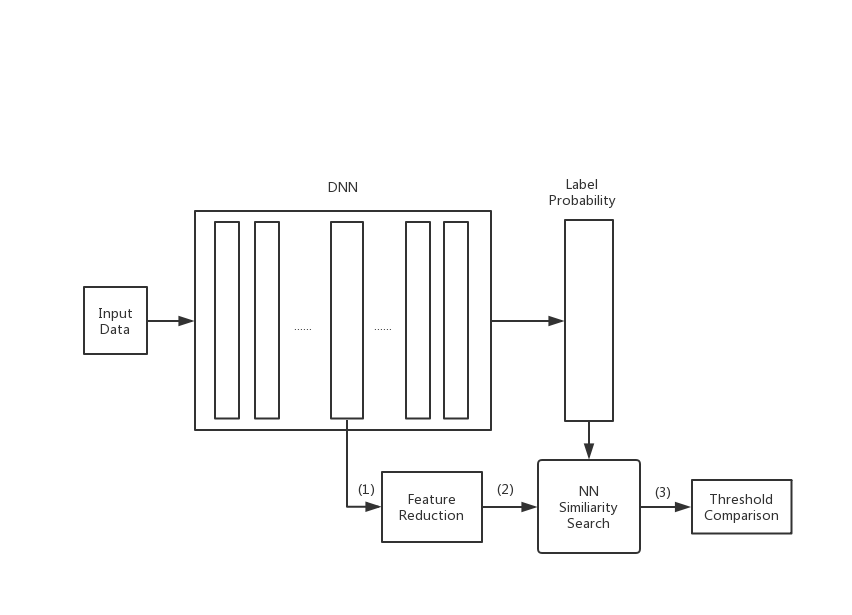
\includegraphics[width=3.2in,height=2.5in]{fig//fw1.jpg}
	\caption{Framework of Adversarial Samples Detections}
	\label{deepfeature}
\end{figure}

\subsection{Deep feature based feature represention and reduction}	
%当下,深度学习功能强大,效果明显,取得了令人瞩目的成绩,深度学习之所以取得这么大的成功,一部分的原因就是,通过搭建足够深的网络和足够多的神经元,可以将原始数据转换到一个更适合的空间中,获得数据的更好的表示,从而完成在之前特征空间难以处理的线性划分的任务。deep feature不仅是原始数据的更抽象提取,同时也看作是一种数据的压缩,在神经网络的每一层获得数据不同的抽象表示,由点到线,由线到面,完成同LFDA、GEM同样的工作,尽可能的保留原始数据之间的相互关系的同时,减少数据的维度,同时还能放大数据之间差异化的作用。接下来的工作会从训练好的神经网络中获得deep feature,用来替代原来的数据表示,进行之后的来实现权重矩阵的计算、相似度计算。LFDA压缩数据,通过计算出来转换矩阵H,数据通过左乘这个转换矩阵实现压缩,这个转换矩阵只是考虑到了数据与数据之间的协方差这一特性,保持数据间的奇异性,就是压缩前后数据间的协方差保持不变,但是同时会使得对抗样本也被压缩到更小的特征空间中,对抗样本和正常的样本间的距离变小,进行相似度计算的时候,使得误分类的比例上升。为了解决这个问题,采用deep feature,神经网络有着数据足够多的数据元,每一个数据元都是一个转换矩阵,能够保留数据之间更多的信息和数据之间的差异,更好的表示数据。 

Currently, deep learning is powerful and effective, and it has achieved remarkable results. The reason why deep learning has achieved such great success is partly by building a deep enough network and enough neurons, converting original feature to a more abstract space, geting a better representation of the data, and completing the task of linear partition that was difficult to handle in the previous feature space.  Different abstract representations of the data are obtained at each layer of the neural network, while retaining the relevance relationship between the original data as much as possible. 
The output features of the intermediate activation layer are extracted from the pre-trained deep neural network to build a deep feature data set. These layer-by-layer non-linear transformation features often have excellent representation capabilities.

For different data sets, we will first use DNN to train a reliable classifier (classification accuracy is above 95 percentenge), and set different numbers of neurons. We then get different neuron weight parameter matrices, that is, get different dimensions deep feature of data samples. Using the obtained deep feature as represrntion of original data samples, we input it into KNN classifier to calculate the similarity on the feature subspace. 
Under the specified constrained attack budget, perturbation is added to each feature pixel along the direction of maximum loss, which eventually leads to agglomeration effects and misclassified especially in high-dimensional features. 
Therefore, the features dimensionality reduction method and the parameterless discrimination model can play a certain role in this attack \cite{carrara2017detecting}.
By comparing the similarity scores between the deep features in the same classes, we can make a valid and reliable judgement. We also can operate feature dimensionality reduction method on obtained deep feature as done on raw data, such as Local Fisher Discriminant Analysis \cite{sugiyama2007dimensionality}.

Based on the above feature processing, we expect the new feature representation to have better trade-off between discrimination and robustness of row samples, and it is more friendly to parameterless models based on spatial distance metrics as showed in Eq. \ref{dis-metric}:
%当然,也可以在学习到的deep feature上做LFDA、GEM压缩。
%之前的方法:LFDA引入了亲密度矩阵,亲密度矩阵,两个样本之间的亲密度,样本间距离足够小,同时样本的邻居之间的距离足够大,则样本间足够亲密;为样本间距离加上了放缩参数,相当于是权重参数,来区别样本间的直接的编辑距离。
%同一个类中的数据样本数量越大,两个样本间通过定义计算出来的亲密度是要大于实际亲密度的,因为样本的数量很大,例如在一个宗亲的地区中,人与人之间的亲密度就并没有在美国的两个中国老乡之间来的亲密;亲密度矩阵是为了计算Slw和Slb,Slw和Slb用来计算映射矩阵T,就是压缩变换矩阵,就是使得投影后的数据保持类内的数据方差足够小,足够密集;类与类之间的中心足够远,类之间足够的分离这一目的。GEM是使得映射后的数据保持最大的方差,数据之间足够的分散,奇异化。
\begin{equation}
\begin{aligned}
Distance\left(\boldsymbol{V}, \boldsymbol{x}, \boldsymbol{X}_{i, j}\right)=\left\|\boldsymbol{V} \boldsymbol{x}-\boldsymbol{V} \boldsymbol{X}_{i, j}\right\|_{2}
\end{aligned}
\label{dis-metric}
\end{equation}
%其中矩阵V就是LFDA或者是GEM计算出来的用来压缩和降维转换的
The $V$ is the transformation matrix based on Local Fisher Discriminant Analysis or the Generalized Eigenvector Method, $x$ is the input test sample and $X_{i,j}$ are the data samples of class $i$ in the training set. The projection transformation matrix $V$ is designed to make the data samples in training set closer of the same class, while samples from differet class are separated in the projected subspace. 

\subsection{Nearest space classifier - all samples considered k nearest neighbors similarity search}
%KNN算法是在整个训练数据集上找到k个距离最近的sample作为待分类样本的邻居,这样search邻居的方法是简单高效的,但是也是容易受到攻击的,因为在这样的场景下,待分类样本的k邻居范围内的数据分布很混乱,数据的multimodality特性,以及数据样本的随机性,不同类别的数据也会在相同的field中一起出现,这时候的分类结果就会有很大的随机性了。
The KNN algorithm finds the $k$ nearest samples in the entire training data set as the neighbors of the sample to be classified, so the method of searching the neighbors is simple and efficient. But it is also vulnerable. For example, the $k$-neighborhood range of the sample to be classified is full of different labeled samples. Since the multimodality and randomness of the data samples are, different classes of data will also appear together in the same field.
This scenario shows that the data has universal multi-modal properties, and some characteristics of the data are usually scattered in multiple samples, and these samples deviate from each other and do not exhibit the characteristics of cluster. Therefore, in classification discrimination based on neighborhood of test sample, considering more data samples can often obtain more general information for each category, and it is robust to classification tasks.
%本文提出两种可行的方法,去论证上面提到的设想。一是当进行KNN查找的时候,不在整个训练数据集找到K个邻居,而是在数据集的每一个类别的子空间上查找待分类样本的K个邻居,最后每个类别的K个邻居根据相似度得出KNN score,score最高的类别就作为待分类样本的类别。另一种是借鉴NS算法的设想,将数据集中每个类的样本考虑在内,通过一个拟合参数得到拟合出来最接近的y,拟合残差最小的类别作为待分类样本最后的类别。

This paper proposes two feasible methods to demonstrate the ideas mentioned above. 
First, when searching $k$ nearest neighbors, neighbors are not found in the entire training data set but in the subspace of each class, that is, we find $k$ neighbors in each subclass. Finally $k*L$ nearest neighbors of a instance $y$ to be classified are based on the smallest cumulative sum distance $l_{i}(\boldsymbol{y})$ to each subspace among all classes $l_{i}(\boldsymbol{y})=\min_{i \in \{1,\dots,L\}}\sum_{1}^{k}\left|x_{y}^{(l)}-X_{i}^{(l)}\right|^{p}$, and we assign $y$ to the class $i$, $L$ is the total amounts of all classes, we defined the method as SK-NN.
The other is based on the idea of the Nearest Space algorithm \cite{liu2011k}, all data samples $\boldsymbol{X}_{i}=\left[\boldsymbol{x}_{i, 1}, \ldots, \boldsymbol{x}_{i, n_{i}}\right]$ of class $i$ can expanded a feature subspace as the basis, we no longer calculate the distance as the similarity between the data samples, but calculate the distance between the test sample and the feature subspace spanned by the training data set of each class and the lable of $y$ is that has smallest distance one. We call the method as AK-NN. 

Different from traditional using the fixed $k$ neighbors as the final criterion, this paper calculates the test sample $y$ among all the samples of each class in the training data set as Eq. \ref{distance_metric} to obtain the distance similarity. That is to say, using all the training data in each class to fit $y$, among all the $l_{i}(\boldsymbol{y})$ which have the smallest residual with the original y, $i$ is the final class label, $\phi(\boldsymbol{y})$ indicates deep feature extracted from neural networks.	
\begin{equation}
d_{i}(\boldsymbol{y},X_i)=\min _{\boldsymbol{\alpha}_{i} \in \mathbb{R}^{n}_{i}, i \in\{1, \ldots, K\}}\left\|\phi(\boldsymbol{y})-\phi(\boldsymbol{X}_{i}) \boldsymbol{\alpha}_{i}\right\|_{2}
\label{distance_metric}
\end{equation}
%y是向量,第i类中的所有数据组成一个矩阵Hi,为了能够比较,需要将矩阵乘以一个拟合向量a,这样矩阵就变成向量,可以进行向量之间的比较了。	
%为了避免过拟合,添加L2正则化项:
%带正则化项的nearest neighborhood算法是,通过一个类的所有对象,一个拟合向量和一个待测样本这三个元素,通过梯度下降的方法找到最优的拟合向量,计算拟合出来的样本和真实的待测样本之间的残差,具有最小残差的拟合向量的类就是待测样本的最终类别。不同于knn的找到k个邻居,就可以确定最终的类别。	
To avoid overfitting and smooth model obtained from the training process of back propagation, add the $L2$ regularization term:	
\begin{equation}	
d_{i}(\boldsymbol{y},X_i)=\min _{\boldsymbol{\alpha}_{i} \in \mathbb{R}^{n}_{i}}\left\|\phi(\boldsymbol{y})-\phi(\boldsymbol{X}_{i}) \boldsymbol{\alpha}_{i}\right\|_{2}+\lambda\left\|\boldsymbol{\alpha}_{i}\right\|_{2}^{2}
\label{distance_metric_withoutoverfit}
\end{equation}

	
%本文分别的在每个类的子集上进行相似度计算,找到每个类上的邻居,这样既可以并发的计算每个类的相似度,最终的分类标准是根据每个类的邻居的得分,最终得分最高的邻居的类作为待测样本的类。这样可以考虑到更大的数据分布,同时也能检测对抗样本。

Based on the above design, there is another advantage, we can search the nearest neighbors in each subclass in parallel on a multi-core machine, so that the  time-consuming computing similarity distances of each class can be reduced to some extent. The final classification criterion is based on the score of nearest neighbors of each class. The class of the neighbor with the highest score(inverse of similiarity distance value) is the class of the sample to be classified. By this way, it is possible to take the multi-model nature of the data and the distribution differences of the data samples into consideration, and detect the adversarial sample finalllty.

%设计得分计算的方法:待测样本在深度特征空间上同每个类(k个类)的所有样本进行比较,得出待测样本关于每个类的分值,那么待测样本y属于类别i的概率就是

Designing similarity score calculation method is listed as follow:
The sample to be classified $x$ is compared with all other samples $X_{i}$ of each class $i$ ($i \in (1,L)$ classes) in the deep feature space and KNN classifier assigns lable $y$ according to the ordered $k$ neighbors $Neighbors(x, X_{i})=\left\{\left(x_{1}, y_{1}\right) \ldots\left(x_{k}, y_{k}\right)\right\}$ to test sample $x$, neighbors $\left(x_{k}, y_{k}\right)$ are calculated and searched according to the predefined two methods SK-NN and AK-NN as Eq.\ref{distance_metric_withoutoverfit}. Obtained all the distances between test $y$ and nearest neighbors, we can get a score distribution, then the probability that the test sample $x$ belongs to category $i$ is $\Pr(x = i)$ as Eq. \ref{probability}. 

\begin{equation}
\Pr(x = i) = 1 - \frac{\sum_{i=1}^{K} distance(x,x_i) D(y_i = i) }{ Neighbors(x,X_i)}
\label{probability}
\end{equation}

When the residual of $distance(x,x_i)$ is smaller, the probability of sample $x$ labeled as $\Pr(x = i)$ is more confident and we regard $distance$ as a weight parameter. Here we use the distance value to represent it, but it can also use other forms to represent it, $D(y_i = i)$ is an indicator function, when the condition is true, output 1, otherwise output 0. When it is greater than a certain threshold, we think it is trustworthy.	
%\begin{equation}
%g(x)=\left\{\begin{array}{ll}{1} & {\text { if } %\eta(x)=\operatorname{Pr}(y=i | x) \geq threshold} \\ {0} & {\text { %otherwise }}\end{array}\right.
%\label{threshold}
%\end{equation}
Of course, under different $L_p$ distance calculation on the obtained deep feature with the LFDA and GEM method we can get different $\Pr(x = i)$. This is the basis we use to determine whether it is an adversarial sample.

\subsection{Adversarial samples dection}
%deep feature是数据的抽象表示,我们用deep feature进行相似度比较,在每一个特征子空间上都会得到一个概率值,如果通过KNN计算出来的概率值符合正确分类的result,即使正确的分类不一定会有最大的概率值,但是如果计算出来的概率值很小,明显的出现区分的情况,那么这个样本就可能是一个对抗样本了。
First, we are based on a trained deep neural network which structure is designed as eight layers composed of convolution layers with max pooling and fully connected layers refered to \cite{sermanet2013overfeat}. 
We choose the fifth layer of the network structure as the source of deep features, and the last layer as the output layer, and output the probability distribution vector of the category of the test sample, so that we can get a corresponding deep feature dataset of the training dataset.
Based on the data representation obtained from the deep feature, we input it into a fast-computing non-parameter neighbor discriminant model. We can get the nearest neighbor similarity score based on this distance similarity model, which is compared with the result vector of the DNN. If the confidence score is substantially positive correlation with the result vector, we can consider the test data to be clean. If the similarity score of the discriminant model is below a certain threshold, we consider the test data sample to be attacked and it is an adversarial sample. The classification results are unreliable and discarded.

In order to ensure the robustness and quality of the classification results, and considering the perturbations accumulation of various feature dimensions in a high-dimensional feature space, we designed a compression and reduction stage of deep feature. In the feature compression phase, according to the categories to which the deep features belong, and the visual similarity between the categories, we use the GEM method and the LFDA method to design the compression transformation matrix $V$ as shown in Eq. \ref{matrix} and optimize the data representation.
\begin{equation}
\boldsymbol{V}=\underset{\boldsymbol{V}}{\arg \max } \frac{\boldsymbol{V}^{T} \boldsymbol{M}_{i} \boldsymbol{V}}{\boldsymbol{V}^{T}\left(\boldsymbol{M}_{j}+\frac{\gamma}{d} \operatorname{trace}\left(\boldsymbol{C}_{j}\right)\right) \boldsymbol{V}}
\label{matrix}
\end{equation}
where $V$ is the obtained compression transformation matrix, $M_i$ represents the difference between the data we want to enlarge, including singularity, covariance or the spatial distance between categories, and $M_j$ is the characteristic feature of the data we want to aggregate, which can be spatial distance within the class, $\frac{\gamma}{d}$ is a scaling parameter and $d$ is the feature dimension of the data sample.

Next, we need to calculate the similarity for the features we have processed, and find neighbors to assist decision-making. As we all know, the KNN model based on the $L_p$ distance is very sensitive to the transformation (common inversions, translations, rotations and etc.) between data samples, so we employ the improved tangent distance based on \cite{simard1998transformation} to measure the distance between data samples under the transformation space. 
In the method framework proposed in the previous chapter, we use two schemes to determine the domain of the neighborhood, and accumulate the nearest neighbor distance in the category subspace as the similarity score $S(x,X_i)$. The probability $ \ Pr (x = i) $ (distribution of similarity scores in different classes of feature subspaces) is used as a sign of the confidence of the classification result, and the output layer of the deep network is compared to determine whether it is an adversarial sample.

%阈值是一个需要多次实验比较和权衡后的选取的超参数,如果我们选择的阈值过大,那么一些置信度较低的正常样本就会被分类成对抗样本,如果我们选择的阈值过小,那么就可能将对抗样本分类成正常的样本,都影响模型的实用性。
The threshold associated with the $s(x, X_{i})$ is a hyperparameter that requires multiple experimental comparisons and trade-offs. If we choose a too large threshold, then some normal samples with low confidence scores will be classified as adversarial samples, that is False Negative(FN) in the binary classification problem. If we choose a too small threshold, the adversarial samples will escape the detection of the classifier model and be classified into normal samples, that is False Positive(FP), which will affect the practicality of the model.
The choice of the probability threshold is a trade-off to balance the problem above, the choice of our threshold needs to take into account the ratio of True Positive(TP) and False Positive for the final result, TP is normal sample that is classified as a normal sample correctly, we need to ensure that as many normal samples as possible are correctly classified.


\section{Performance Evalution}	
%KNN分类算法的问题:1.两类数据存在明显的边界情况下,在内部分类效果很好;但是在分类边界处的分类效果急剧下降;
%实验目的:二分类问题,一个样本是否是对抗样本;
%实验内容:1.不同距离公式:余弦相似度/欧式距离下,二分类结果
%实验内容:2.存在对抗样本下的分类准确性,混淆矩阵,ROC曲线确定最优的概率划分	
%实验内容:3.不同的特征表示/压缩方法下,二分类结果
%实验内容:4.不同数据集下,二分类结果
%实验指标:二分类的分类结果:准确率,精确率, 召回率;多分类一般只看准确率
In this chapter, we will conduct experiments to evaluate the effectiveness and robustness of our models. The proposed method has mainly been evalauted as detecting adversarial samples when a normal sample is attacked by Fast Gradient Sign and L-BFGS and to give a confidence score of the result of the classification. When the output of confidence score above the trade-off threshold it means the sample to be classified is normal; otherwise it  indicades the sample is attacked and is an adversarial sample.

We use three datasets: MNIST, CIFAR-10 and Caltech to verify the proposed model. Pictures of objects belonging to 101 categories of the Caltech. It is about 40 to 800 images for per category. Most categories have about 50 images. The CIFAR-10 dataset consists of 60000 32x32 colour images in 10 classes, with 6000 images per class.


Table \ref{tabel_1} shows the results of classification accuracy under different proportions of adversarial samples in the training data set,  $p_{0}$ is with no adversarial samples while $p_{1}$ is with 5 percentage adversarial samples, $p_{2}$ is with 10 percentage adversarial samples, $p_{3}$ is with 15 percentage adversarial samples, $p_{4}$ is with 20 percentage adversarial samples. For the three data sets, the appearance of the adversarial samples did have an impact on the classification task. When the number of adversarial samples gradually increased, the accuracy of the classification decreased significantly. 
\begin{table}
	\centering
	\caption{Classification Accuracy under Adv. Perturbations}
	\begin{tabular}
		{>{\columncolor{white}}rccccc}
		\toprule
		\rowcolor[gray]{0.9}&$p_{0}$&$p_{1}$&$p_{2}$&$p_{3}$&$p_{4}$\\
		\midrule
		CIFAR-10&\multicolumn{1}{>{\columncolor{white}[0pt][0pt]}c}{0.96}&0.88&0.80&0.73&0.62\\
		\midrule
		MNIST&\multicolumn{1}{>{\columncolor{white}[0pt][0pt]}c}{0.95}&0.86&0.82&0.70&0.59\\
		\midrule
		Caltech&\multicolumn{1}{>{\columncolor{white}[0pt][0pt]}c}{0.95}&0.96&0.78&0.72&0.60\\
		\bottomrule
	\end{tabular}
	\label{tabel_1}
\end{table}
%在表2中,我们记录下采用不同的判别模型方案下,检测对抗样本的效果。其中基于传统的KNN判别模型是引自【】的工作,我们可以看到无论是准确率相比较与没有使用判别模型的深度网络还是有所提升的,但是召回率较低,这也说明了存在一些FP的问题。接下来的4行,分别是1,2,3,4方法,基于重新设计的距离度量以及数据压缩方法,在准确性和召回率上都取得了较为明显的提升,尤其是在召回率上,较好的解决了FP的问题,在后面的实验中也会论证我们的这一成果。 其中使用AK-NN和LFDA数据降维方法获得最佳的性能。 
In Table \ref{table_2}, we record the effect performance of detecting adversarial samples with different discriminant model schemes. Among them, the traditional KNN discriminant model is quoted from the work \cite{carrara2017detecting}. We can see that the precision rate is improved compared with the deep network without the discriminative model, but the recall rate is relatively low, which indicates that the model has the problems of False Negatives, that is, it will treat clean inputs as adversarial samples and discarded totally, which needs to be improved. 
The next four lines are the SK-NN and Ak-NN methods proposed in this paper. Based on the redesigned distance measurement and data compression methods, the precision and recall rate have been improved significantly, and the problem of False Negatives has been solved better. In the subsequent experiments, we will continue to demonstrate our improvement of this achievement. Among them, Ak-NN with LFDA data dimensionality reduction method obtains the best performance.
	
\begin{table}
	\centering		
	\caption{Classificaton Prediction Performance Comparison.}
	\begin{tabular}{|c|c|c|c|c|} \hline
		\multirow{2}*{Method} &\multicolumn{2}{c|}{FGS attack} & \multicolumn{2}{c|}{L-BFGS attack}\\ \cline{2-5} 
		&Precision& Recall & Precision&Recall\\\hline
		KNN&0.7324&0.618&0.7371&0.6142\cr\hline
		SK-NN&0.7621&0.6685&0.7163&0.6762\cr\hline
		AK-NN&0.7831&0.7222&0.7843&0.7527\cr\hline
		AK-NN with GEM&0.8142&0.7599&0.8695&0.7984\cr\hline
		AK-NN with LFDA&0.8335&0.7933&0.8386&0.8148\cr\hline
	\end{tabular}
	\label{table_2}
\end{table}

%添加实验
%1.不同的特征降维方案在同一数据集上的表现情况
%2.选择一个ensemble的方案,测试在不同数据集上的效果
%3.不同的阈值选择,对分类准确性的影响情况

\begin{figure}
	\centering
	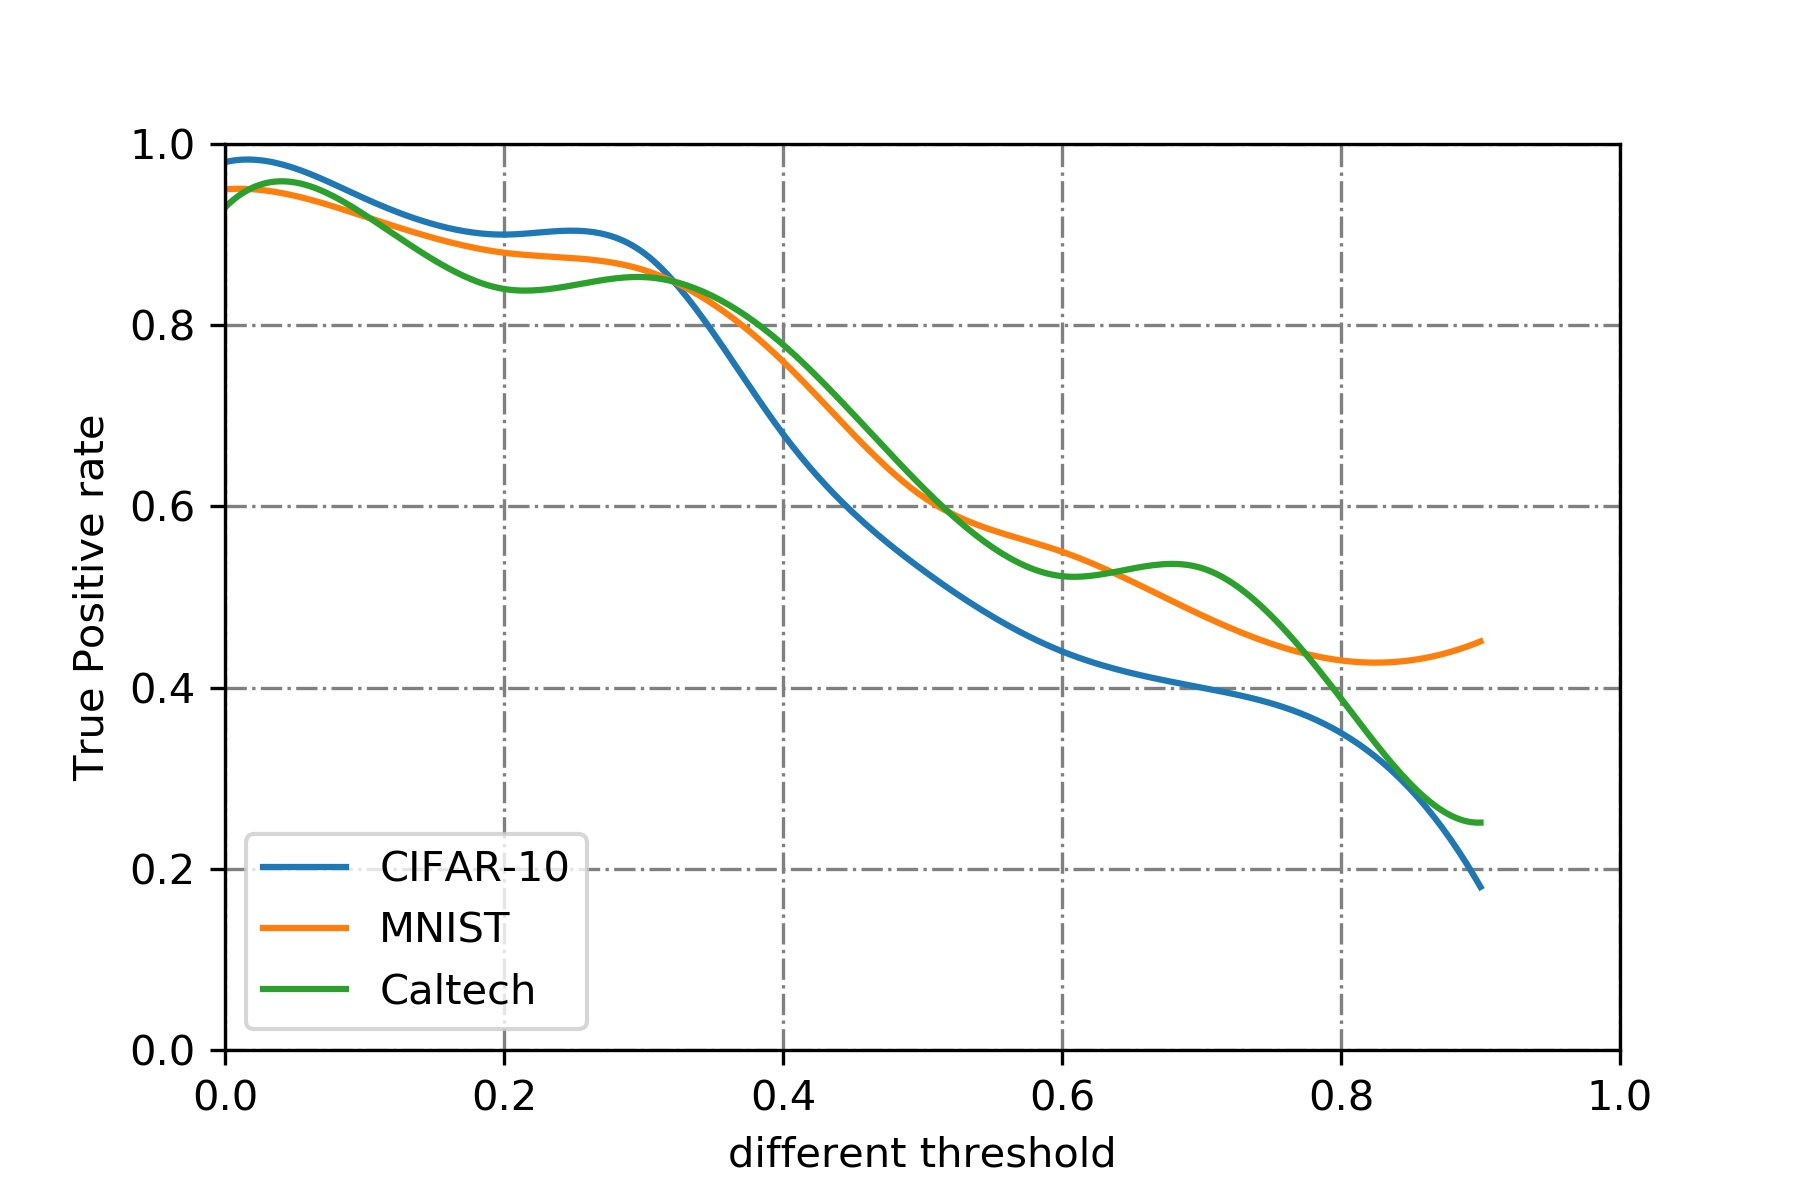
\includegraphics[width=3in,height=2in]{fig//222.jpg}
	\caption{The Ratio of TP under Different Thresholds}
	\label{Differrnt dataset}
\end{figure}
%我们在3个数据集上进行了实验,测量了在不同的阈值情况下,本文提出的模型在分类TF样本的情况。随着阈值的增大,从图中我们可以看到不同的数据集下降的趋势是不一样快的,这说明不同的数据集,针对数据集中的正常样本生成的对抗样本,数据集本身也具有一定的鲁棒特性。随着阈值变大,相似度分数大于选定阈值的才能确定为是正确的分类样本,我们发现当阈值设置为0,6时,我们仍然能够保留下50%的正常样本在MINIST和Caltech,但是CIFAR-10数据集中只保留了40%的正常样本了,剩下的都因为不够相似而被误判成对抗样本。因此研究这些本身就具有很好的鲁棒性的数据集,从这些数据集中样本抽出的深度特征对于对抗的扰动不敏感,有助于进一步提升模型对于对抗样本的防御性能。
We performed experiments on three data sets and measured the proportion of TP in the classification results under different threshold conditions. In Fig.\ref{Differrnt dataset} as the threshold increases, we can see that the trend of decrement is not as fast as each other, which means that different data sets, also has original robustness naturally, as the discrimination threshold increases, the data set that can retain more True Positive samples is a more robust data set for research. We find that when the threshold is set to 0.6, we can still retain the next 50 percent of the normal sample in MINIST and Caltech, but only 40 percent of the normal samples are retained in the CIFAR-10 dataset, and the rest are incorrectly classified as adversarial samples because they are not with confidence scores enough assigned by the AK-NN. Therefore, these data sets which are inherently robust are studied. The deep features extracted from the samples in these data sets are not sensitive to the malicious disturbance, which helps to further improve the defensive performance of the model against the adversarial sample.


\begin{figure}
	\centering
	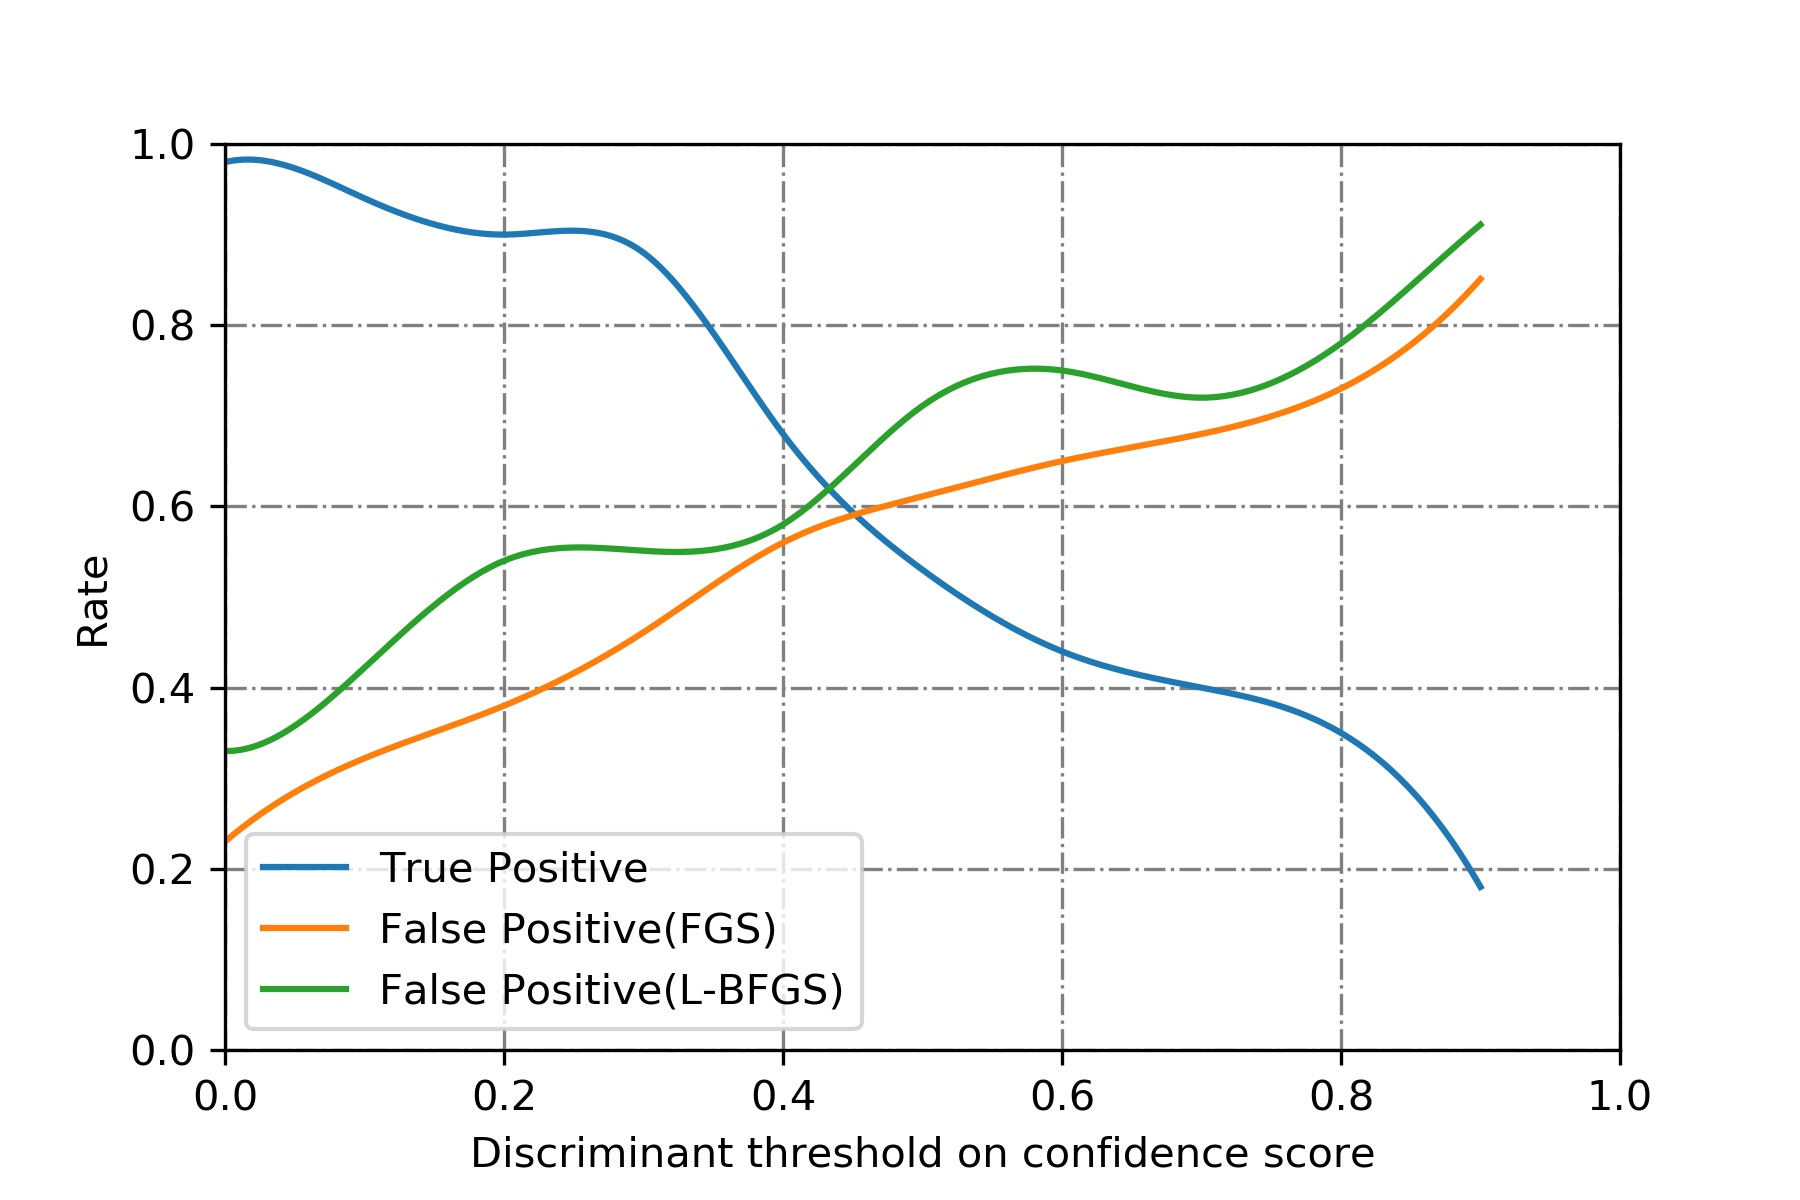
\includegraphics[width=3in,height=2in]{fig//111.jpg}
	\caption{TP and FP Rates with Different Threhold on Confidence Score}
	\label{TF Rate}
\end{figure}
%在下文中,我们关注基于deep feature计算得到的类别相似度得分。 在图3中,我们统计了对于正确分类的真实图像和对抗对抗图像错误分类成正确图像在不同的判别阈值下的分布情况。 结果表明,不必使用很低的阈值就可以,可以正确地过滤出L-BFGS和FGS产生的对抗性例子,同时保留超过98%的正确图像正确分类。之前的工作中\ref{carrara2017detecting}只能使用低小的阈值,显示DW-kNN分数在分类图像时不会有效,本文提出的方法有了较大的改进。
Then we devote mind to the similarity score calculated based on the best AK-NN with LFDA. In Fig.\ref{TF Rate}, we show the rate distribution for True positive and false positive rates with different discrimination threhold on confidence score. The results show that it is not necessary to use a very low threshold such as 0.2, and the adversarial samples produced by L-BFGS and FGS can be correctly filtered out more than 50 percent while retaining more than 90 percent of clean data samples classified properly. In the previous work, can only use low thresholds below 0.2, and so the similarity scores are not effective when classifying images. The method proposed in this paper has been improved.

\begin{figure}
	\centering
	
	\subfigure[]{
		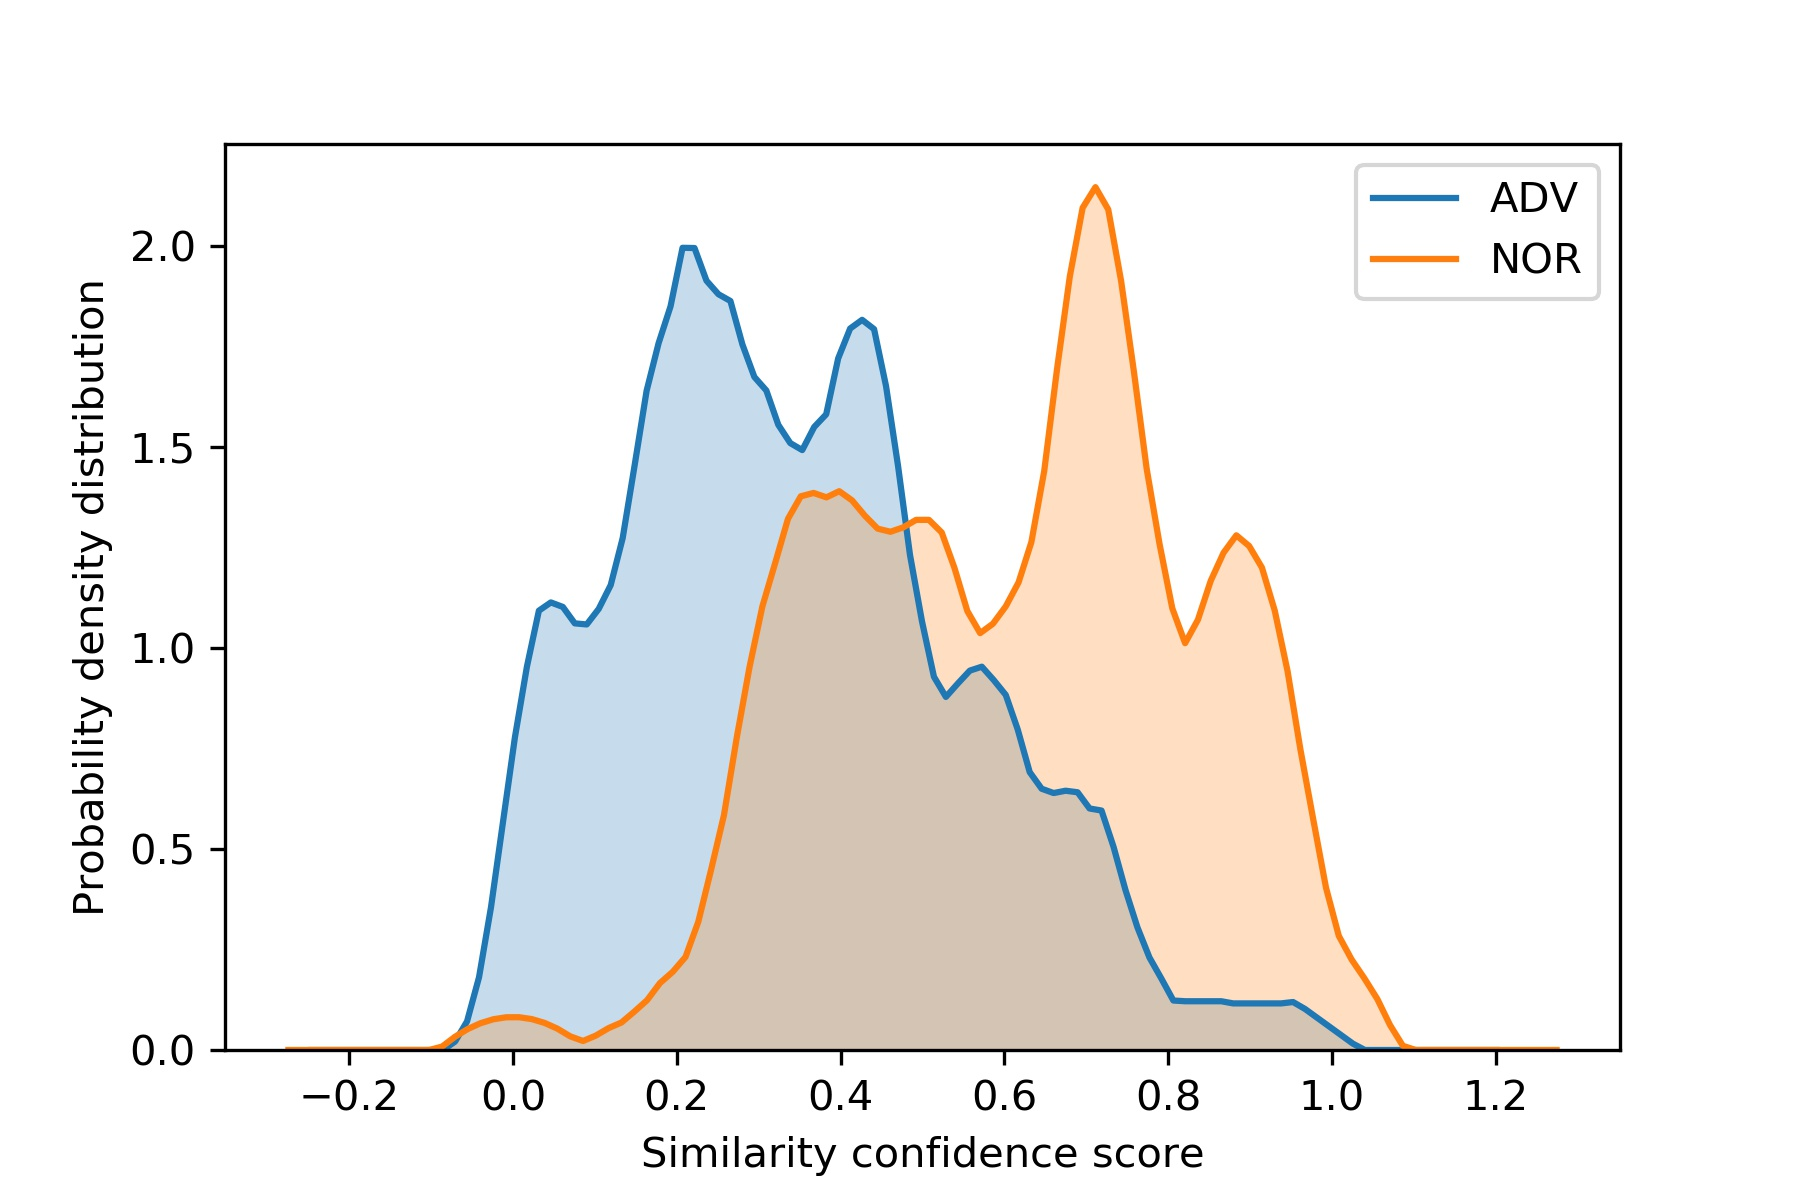
\includegraphics[width=3in,height=2in]{fig//distri1.jpg}
		%\caption{fig1}
		\label{density distribution1}
	}
	\quad
	\subfigure[]{
		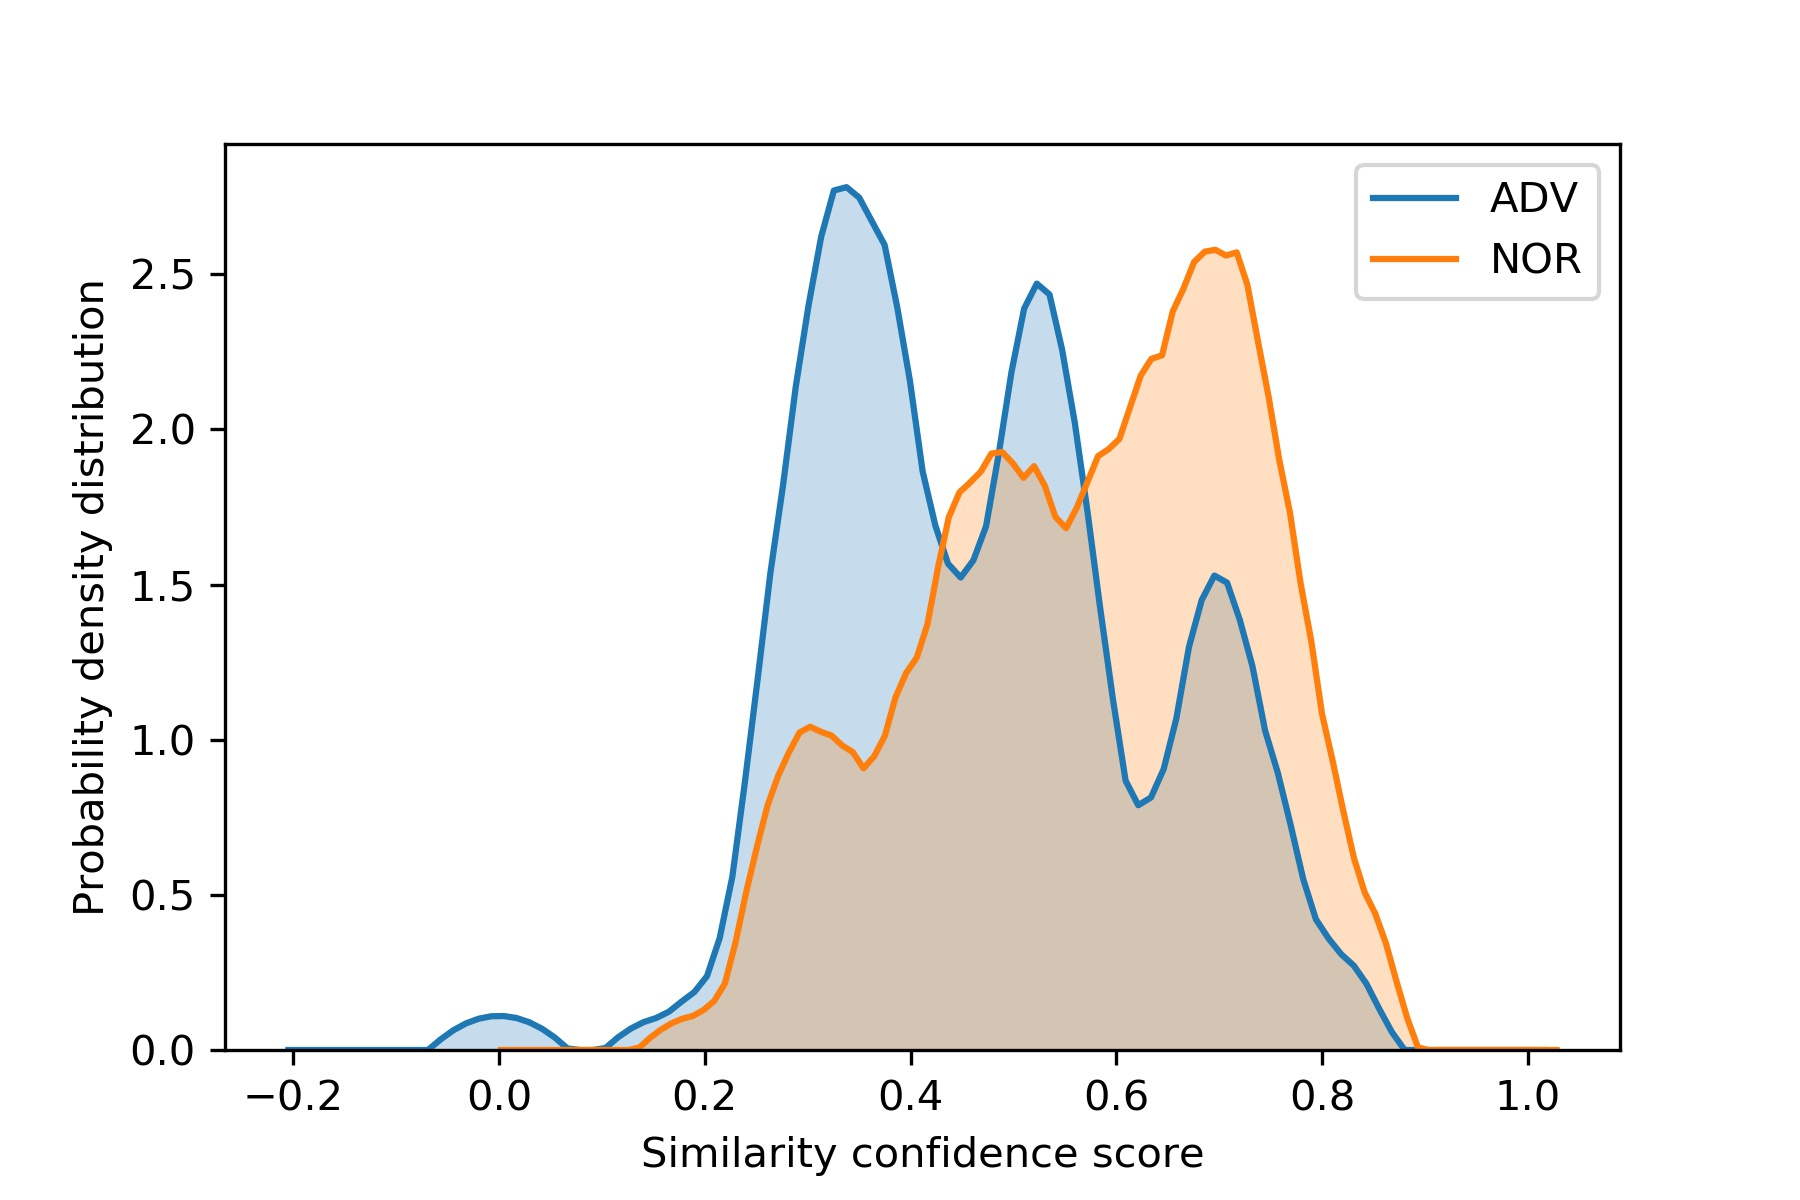
\includegraphics[width=3in,height=2in]{fig//distri2.jpg}
		\label{density distribution2}
	}
	
	\subfigure[]{
		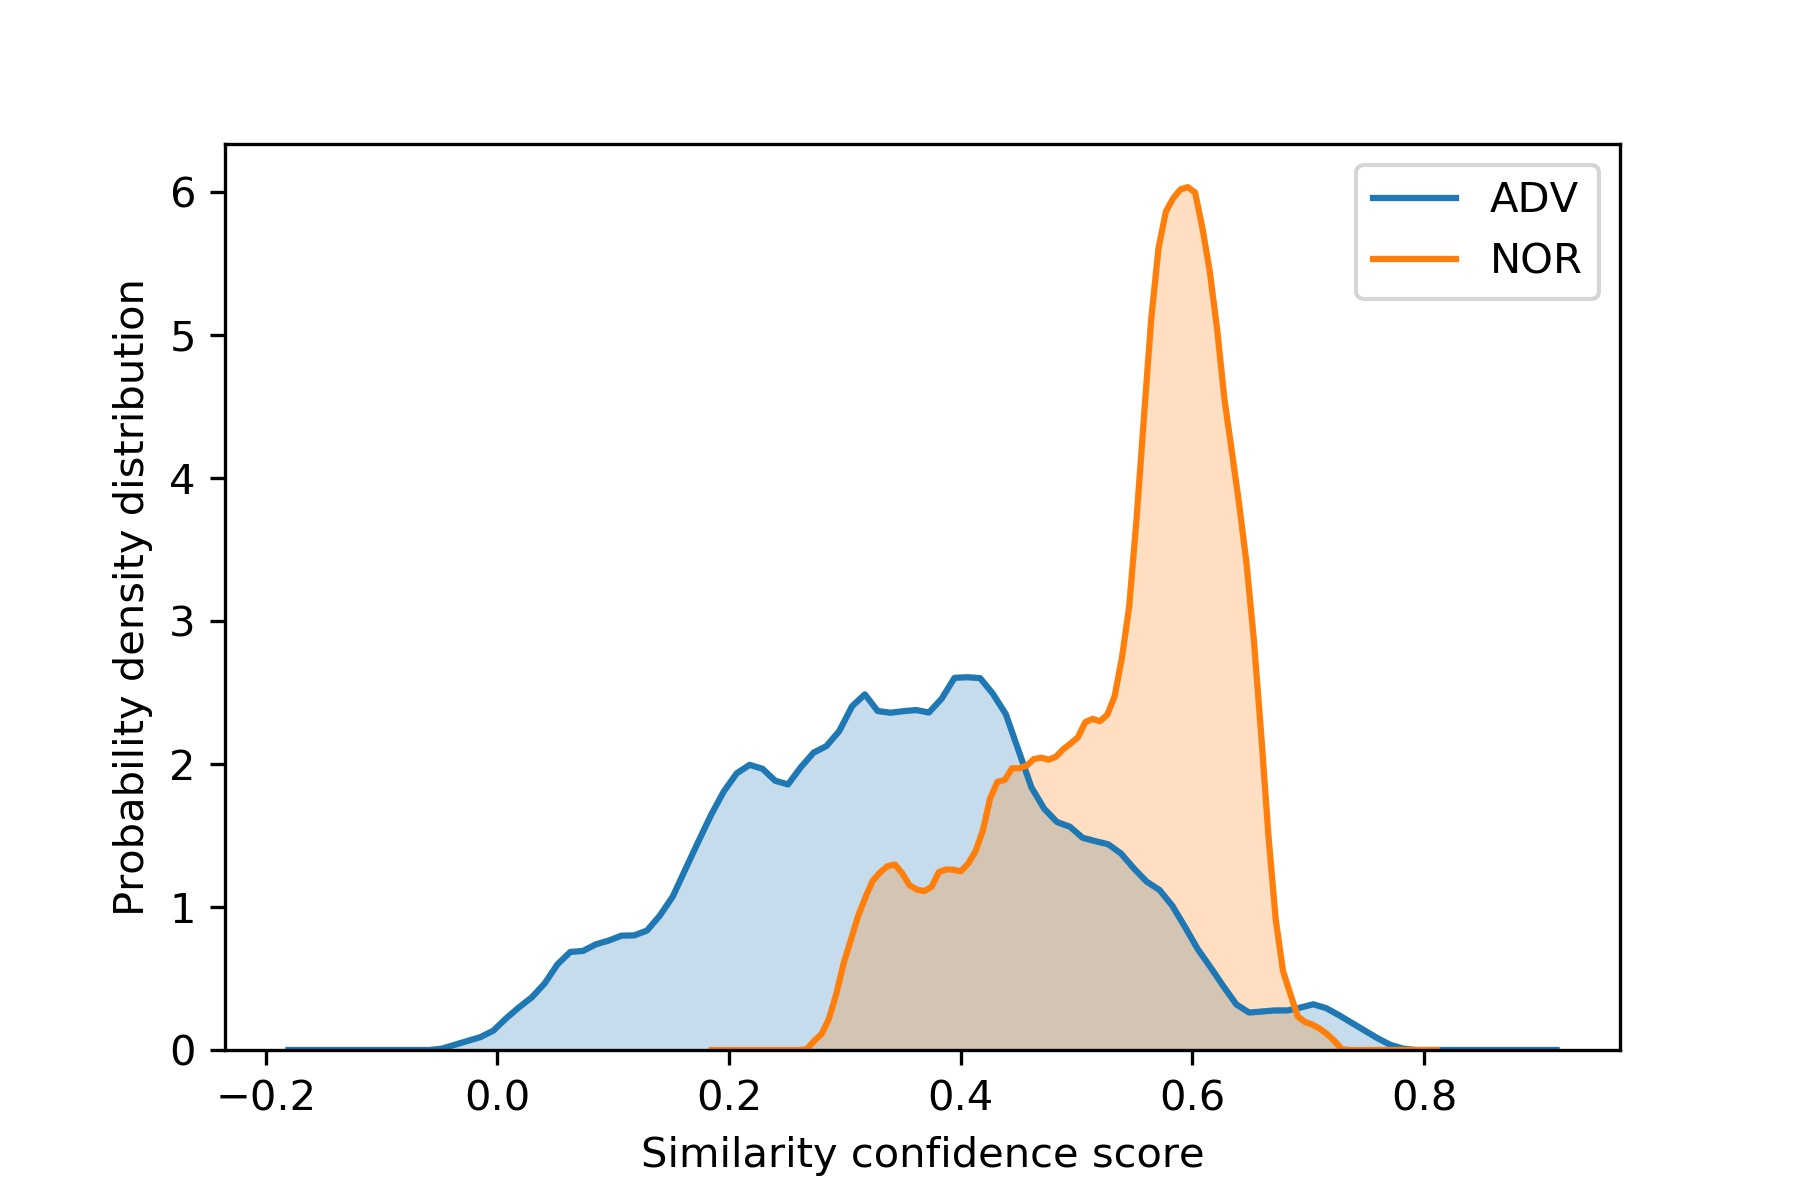
\includegraphics[width=3in,height=2in]{fig//distri3.jpg}
		\label{density distribution3}
	}
	
	\caption{Scores Distribution for the Adversarial and Clean Samples with the AK-NN under Different Data Sets.}
	
	\label{density distribution}
\end{figure}
%但是在图片2中我们的实验结果不是很理想,从图中我们可以观察到有一定比例的对抗样本同样具有较高的置信度分数,尤其是在分类的样本具有较多的类别情况下,在二分类的任务重,往往能取得更加出色的检测对比结果,因为需要同所有的特征子空间计算相似度,有时候就会弱化了泛化了对抗样本的检测。但是通过比对这些分类错误的样本及其最近邻样本,我们发现那些有着很高置信度分数的对抗样本,通常反映出类间的视觉模式上的相似性,而这些相似性与输入图像的对抗性无关,类似于通过生成模型生产出了一批真实的样本。

From the experimental results under three data sets in Figure \ref{density distribution}, we can see that the confidence score given by the discriminant model has a clear boundary, which illustrates the effect of our work. Our method can better distinguish between the adversarial sample and clean sample.
Most of the similarity scores of the adversarial samples are concentrated at around smaller value and the normal samples have similarity scores greater than the value of adversarial samples.
In Figure \ref{density distribution2}, we find that a high proportion of the adversarial samples also have higher confidence scores, especially in the case that the classified samples have more categories more than 100. It is necessary to calculate the similarity with all the feature subspaces, and sometimes the generalization of the adversarial sample detection is weakened. But by comparing these misclassified samples and their nearest neighbor samples, we find that those misclassified samples with very high confidence scores usually reflect the similarity in visual patterns between classes, and these similarities are irrelevant the input adversarial samples which is likely producing a batch of 'real' samples by the generating models.
Overall all the results show, that based on the method proposed in the paper, the adversarial sample can be effectively detected from the normal sample, so some simple metrics on those densities could be computed on-line to detect against a malicious attack, rejected the sample, and improved robustness of the classification model.


	\section{Discussion And Conclusion}
%分析实验的结果,通过以上的实验,我们可以发现以下的一些结论和事实。首先,我们通过向原有的正常的没有添加对抗扰动的数据集中注入特意生成的对抗样本,knn分类模型的分类准确性出现了十分明显的下降,这说明knn这一类无参数的、特别依赖数据的机器学习算法对于对抗样本是敏感的,也是容易被对抗样本干扰的。其次,数据的不同的表示形式,也就是说通过降维、映射、转换等方式,改变原始数据的特征空间,在不同的特征空间下的表示具有不同程度的鲁棒性,选择抽象的、不同的维度表示的方式代替原有的数据表示能够一定程度上防御对抗样本的攻击,或者说是让对抗样本更难的生成。最后,针对数据具有多模态、集群分布、传播的性质,在分类的时候,按照不同类别的分布以及每个类别的特征子空间上进行相似度的计算,计算出来的相似度分数作为一种可信程度给最终的结果打分,能有效的检测出对抗样本,也就是说分类的结果更加可信,错误分类的比例下降。
%存在接近的相似度分数,例如88.7和89.3,往往这些类别之间存在模式、visual上的相似,因此这是一类难以区分的分类。但是,人类在这一模式、视觉相似的分类任务上,正确率也不高。	
%本文提出的方法能够detect到攻击DNN的对抗样本,利用就算deep feature和特征子空间的相似度,能够很好的解决这一问题。
%本文中,我们提出了一种新的用来检测对抗样本的方法,不同于以往的工作,我们将目光投向了应用更加广泛,原理更加简单的无参数化方法KNN上面。首先,我们发现现有的关于KNN的工作没有很好的考虑到对抗样本存在的隐患,导致有的情况下我们的分类结果是不可靠、不可信的,是存在漏洞的.并且进行实验也论证了这种现象,当存在一定数量的对抗样本的时候,我们KNN模型的分类准确性会有一个明显的降低;其次,我们利用当先最火热的特征提取和表示方法deep feature作为我们的数据的表示,利用这种抽象的数据表示方法,比原始的数据表示更powerfu结合基于特征子空间的近邻相似度计算方法,能够对分类结果的进行有效的保证,使得最终的分类结果可靠有效。我们不仅可以检测出被攻击的样本,同时还保证了正常的样本的分类性能,并没有将所有的样本都认为是对抗样本来降低了系统的实用性能。
%数据之间的关联关系也是数据鲁棒性的一种保障,KNN在进行分类预测的时候,需要通过计算出来的邻域内的样本的标签的分布来确定,如果进行投票决策的邻域很小的话,只需要修改很少的样本就可以达到攻击的效果,但是如果邻域足够大的话,攻击的成本就会很大,因为需要修改邻域内的样本的数量会随着邻域的增加而增加,这样就会产生攻击效果不佳的对抗样本,对模型带来的影响就会减少。the relational (non-i.i.d.) nature of the data might improve robustness since the embeddings are computed for all nodes jointly, rather than for individual nodes in isolation
%并且,在实验中我们也发现了这样的一种现象,那些在实验中最后很难被检测到的对抗样本,就是具有很好的可信的分数的对抗样本,往往和正常的样本存在大量的相似性和相关性,包括类别本身上的相似以及某些视觉模式上的相似,这在自然界中也是广泛存在的一种现象,例如狐狸狗和狐狸之间,它们属于不同的族群,但是在外貌上存在很多的相似性。
We injected specially generated adversarial samples into the original normal data set, and the classification accuracy of the KNN classification model showed a significant drop. This shows that KNN a non-parameter, data driven machine learning algorithm is sensitive and vulnerable to adversarial samples. Secondly, the different representations of the data, the feature space of the original data is changed by means of dimensionality reduction, mapping, transformation, etc.. The representations of the original data under different feature spaces have different degrees of robustness. Choosing an more abstract, different dimension representation instead of the original data representation can protect against the adversarial attack to a certain extent, or make the adversarial samples more difficult to generate. Finally, for the data with multimodality, cluster distribution, and propagation properties, when classifying and predicting the label, the similarity scores of KNN are calculated according to the distribution of different categories. Based on  the characteristic subspace of each category, as many samples as possible to ensure the integrity and comprehensiveness of the data samples. The calculated similarity score can be used as a kind of credibility judgment for the final result, which can effectively detect the adversarial samples. The classification result is more credible, the proportion of misclassification decreases.

We design a novel method for detecting adversarial samples. Compared with previous achievements, we focus on the non-parameterization method KNN which is more widely used and implement in principle. Our experiment shows when there are a certain number of adversarial samples, the classification accuracy of our KNN model will be significantly reduced. Then, we use the deep feature as the data representation. By using this abstract data representation method, it is more powerful than the original data representation combined with the feature subspace-based neighbor similarity calculation method. It can effectively guarantee the classification result, and make the final classification result reliable and effective. Not only can we detect the sample being attacked, but also we ensure the classification performance of normal samples. We do not exaggerate the proportion of the adversarial samples to reduce the practical performance of the KNN classification.The relational (non-i.i.d.) nature of the data might improve robustness since the KNN similiarity scores are computed for all samples jointly, rather than for individual samples in isolation. When performing classification prediction, KNN needs to refer to the distribution of the labels of the samples in the neighborhood, if the neighborhood of the voting decision is small, the attack effect can be achieved by only modifying a small number of samples. But if the neighborhood is large enough, the cost of the attack will be large, because the number of samples in the neighborhood to be modified will increase as the neighborhood increases and evevtly generate adversarial samples more arduously. This will result in a poor adversarial attack performance, and the impact on the KNN model will be reduced.

%关于如何将对抗样本用于正当目的的问題:通常意义上的对抗样本是一种对人工智能的恶意应用,常被与欺骗、攻击、伪装联系在一起,会对人工智能系统造成极大威胁。而正确地使用对抗样本技术,使其发挥积极作用,这一点需要引起研究者们更多的关注。在隐私保护方面,恶意地利用人工智能系统对用户的上传到网络上的图像数据进行釆集并分析,是对用户隐私的极大威胁。此时可以通过对抗样本技术对图像数据进行伪装或隐藏,欺骗基于神经网络的图像识别系统,从而达到保护用户隐私的目的。对抗样本还可应用于验证码的生成,目前使用神经网络对验证码进行快速高效的识别,这使得网站面临着被恶意破解密码、恶意大规模注册等威胁,针对验证码识别系统生成对抗样本来构建安全的验证码也是对抗样本的正面应用之一。故探究如何巧妙地将对抗样本应用到正当目的也是一个值得研究的问题。
Moreover, we observed the experimental results and found the following phenomenon: some adversarial samples are easily detected by our discriminant model, that is, they have a lower confidence score $s(x,X_i)$; but some adversarial samples are difficult to detect, the confidence scores of the adversarial samples are confusing, either the distributions are roughly uniform without directivity or having a higher probability consistent with the original category by DNN. The second situation deserves our attention, we observe and compare the adversarial samples and the normal samples in the training data set, and we find that these adversarial samples tend to have similar patterns, including similarities in the categories themselves and similarities in certain visual patterns, that is also a widespread phenomenon in nature, such as between Japanese Spitz and white foxes, which belong to different ethnic groups but in appearance there is a lot of similarity on it.

How to use the adversarial sample for the proper purpose: Generally speaking, the adversarial sample is a kind of malicious application to artificial intelligence. It is often associated with deception, attack and camouflage, which will pose a great threat to the artificial intelligence system. However, more attention should be paid to the correct use of adversarial sample technology to make it play a positive role. In the aspect of privacy protection, using artificial intelligence system to collect and analyze the image data uploaded to the network is a great threat to the user's privacy. At this time, we can camouflage or hide the image data through the adversarial sample technology, and cheat the image recognition system based on neural network, so as to protect the privacy of users. Therefore, it is worth studying how to apply the adversarial samples to the proper purpose.

In general, our method has obtained satisfactory results in terms of classification accuracy, scalability, and practicality, and we will continue to expand our research in the next work.


\section*{Acknowledgment}


\bibliographystyle{unsrt}
\bibliography{ref}

%{\includegraphics[width=1in,height=1.25in,clip,keepaspectratio]{1111.jpg}}
\begin{IEEEbiography}[{
\includegraphics[width=1in,height=1.25in,clip,keepaspectratio]{yiren.jpg}}]{Yi Ren}
	received the B.E. degree in computer science and technology from Sichuan University, Chengdu, China, in 2017. He is currently pursuing the M.E. degree in computer science with the Huazhong University of Science and Technology. His current research interests include big data and machine learning.
	
	
\end{IEEEbiography}

\begin{IEEEbiography}[{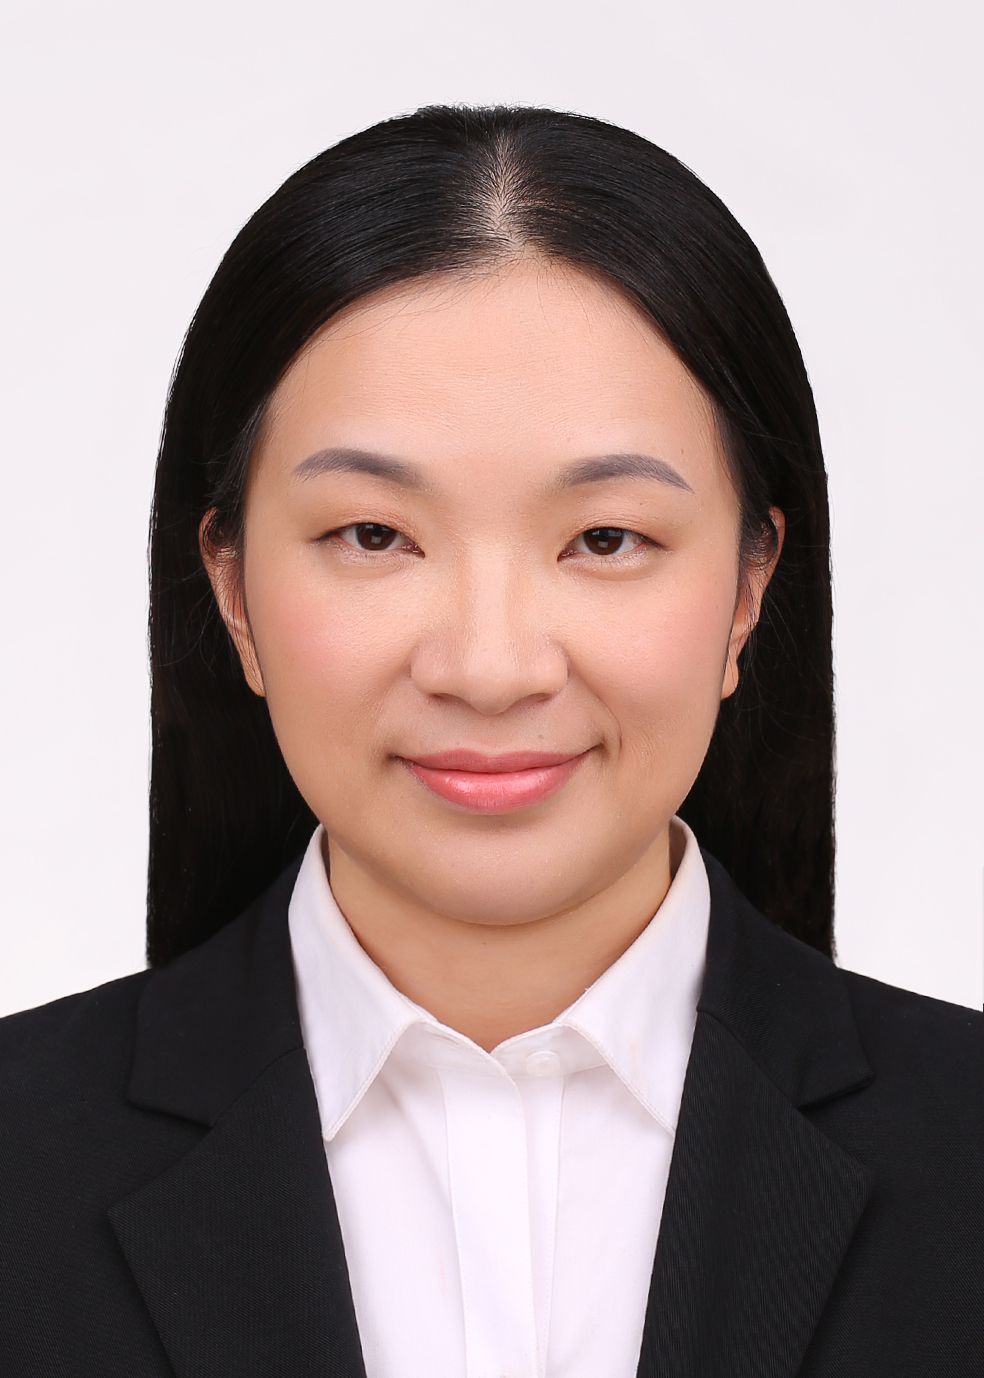
\includegraphics[width=1in,height=1.25in,clip,keepaspectratio]{xiaxie.jpg}}]{Xia Xie} is an associate professor at Huazhong University of Science and Technology (HUST) in China. She received her Ph.D. in computer architecture from HUST in 2006. Her research interests include data mining and big data. Contact her at shelicy@hust.edu.cn.
\end{IEEEbiography}

\begin{IEEEbiography}[{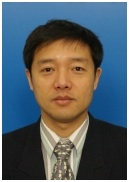
\includegraphics[width=1in,height=1.25in,clip,keepaspectratio]{haijin.jpg}}]{Hai Jin} is a Cheung Kung Scholars Chair Professor of computer science and engineering at Huazhong University of Science and Technology (HUST) in China. He is now Dean of the School of Computer Science and Technology at HUST. Jin received his PhD in computer engineering from HUST in 1994. In 1996, he was awarded a German Academic Exchange Service fellowship to visit the Technical University of Chemnitz in Germany. Jin worked at The University of Hong Kong between 1998 and 2000, and as a visiting scholar at the University of Southern California between 1999 and 2000. He was awarded Excellent Youth Award from the National Science Foundation of China in 2001. Jin is the chief scientist of ChinaGrid, the largest grid computing project in China, and the chief scientists of National 973 Basic Research Program Project of Virtualization Technology of Computing System, and Cloud Security.
	
Jin is an IEEE Fellow and a member of the ACM. He has co-authored 15 books and published over 500 research papers. His research interests include computer architecture, virtualization technology, cluster computing and cloud computing, peer-to-peer computing, network storage, and network security.
	
Jin is the steering committee chair of International Conference on Green, Pervasive and Cloud Computing (GPC), Asia-Pacific Services Computing Conference (APSCC), International Conference on Frontier of Computer Science and Technology (FCST), and Annual ChinaGrid Conference. Jin is a member of the steering committee of the IEEE/ACM International Symposium on Cluster Computing and the Grid (CCGrid), the IFIP International Conference on Network and Parallel Computing (NPC), and the International Conference on Grid and Cooperative Computing (GCC), International Conference on Autonomic and Trusted Computing (ATC), International Conference on Ubiquitous Intelligence and Computing (UIC).
\end{IEEEbiography}

\begin{IEEEbiography}[{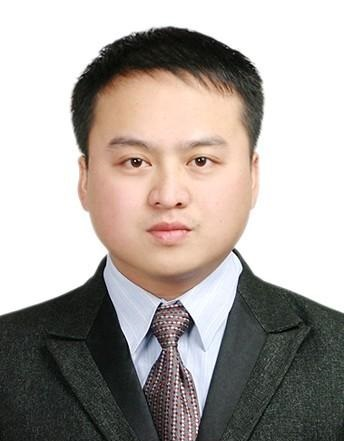
\includegraphics[width=1in,height=1.25in,clip,keepaspectratio]{hanhua.jpg}}]{Hanhua Chen} is a professor at Huazhong University of Science and Technology (HUST) in China. He received the  Ph.D. in computer architecture from HUST in 2010. His research interests mainly include distributed systems and Big Data processing.
\end{IEEEbiography}


\EOD

\end{document}
